%-- coding: UTF-8 --
\documentclass[12pt]{report}
\usepackage[utf8]{inputenc}
\usepackage[left=2.5cm,right=2.5cm,top=2cm,bottom=3cm]{geometry}
\usepackage{fancyhdr}
\usepackage{cite}
\usepackage{url}
\usepackage{sectsty} % Enables custom section titles
\usepackage{graphicx}
\usepackage{verbatim}
\usepackage{latexsym}
\usepackage{mathchars}
\usepackage{setspace}
\usepackage[toc]{appendix}

\setlength{\parskip}{\medskipamount}  % a little space before a \par
\setlength{\parindent}{0pt}	      % don't indent first lines of paragraphs
%UHEAD.STY  If this is included after \documentstyle{report}, it adds
% an underlined heading style to the LaTeX report style.
% \pagestyle{uheadings} will put underlined headings at the top
% of each page. The right page headings are the Chapter titles and
% the left page titles are supplied by \def\lefthead{text}.

% Ted Shapin, Dec. 17, 1986

\makeatletter
\def\chapapp2{Chapter}

\def\appendix{\par
 \setcounter{chapter}{0}
 \setcounter{section}{0}
 \def\chapapp2{Appendix}
 \def\@chapapp{Appendix}
 \def\thechapter{\Alph{chapter}}}

\def\ps@uheadings{\let\@mkboth\markboth
% modifications
\def\@oddhead{\protect\underline{\protect\makebox[\textwidth][l]
		{\sl\rightmark\hfill\rm\thepage}}}
\def\@oddfoot{}
\def\@evenfoot{}
\def\@evenhead{\protect\underline{\protect\makebox[\textwidth][l]
		{\rm\thepage\hfill\sl\leftmark}}}
% end of modifications
\def\chaptermark##1{\markboth {\ifnum \c@secnumdepth >\m@ne
 \chapapp2\ \thechapter. \ \fi ##1}{}}%
\def\sectionmark##1{\markright {\ifnum \c@secnumdepth >\z@
   \thesection. \ \fi ##1}}}
\makeatother
%%From: marcel@cs.caltech.edu (Marcel van der Goot)
%%Newsgroups: comp.text.tex
%%Subject: illegal modification of boxit.sty
%%Date: 28 Feb 92 01:10:02 GMT
%%Organization: California Institute of Technology (CS dept)
%%Nntp-Posting-Host: andromeda.cs.caltech.edu
%%
%%
%%Quite some time ago I posted a file boxit.sty; maybe it made it
%%to some archives, although I don't recall submitting it. It defines
%%	\begin{boxit}
%%	...
%%	\end{boxit}
%%to draw a box around `...', where the `...' can contain other
%%environments (e.g., a verbatim environment). Unfortunately, it had
%%a problem: it did not work if you used it in paragraph mode, i.e., it
%%only worked if there was an empty line in front of \begin{boxit}.
%%Luckily, that is easily corrected.
%%
%%HOWEVER, apparently someone noticed the problem, tried to correct it,
%%and then distributed this modified version. That would be fine with me,
%%except that:
%%1. There was no note in the file about this modification, it only has my
%%   name in it.
%%2. The modification is wrong: now it only works if there is *no* empty
%%   line in front of \begin{boxit}. In my opinion this bug is worse than
%%   the original one.
%%
%%In particular, the author of this modification tried to force an empty
%%line by inserting a `\\' in the definition of \Beginboxit. If you have
%%a version of boxit.sty with a `\\', please delete it. If you have my
%%old version of boxit.sty, please also delete it. Below is an improved
%%version.
%%
%%Thanks to Joe Armstrong for drawing my attention to the bug and to the
%%illegal version.
%%
%%                                          Marcel van der Goot
%% .---------------------------------------------------------------
%% | Blauw de viooltjes,                    marcel@cs.caltech.edu
%% |    Rood zijn de rozen;
%% | Een rijm kan gezet
%% |    Met plaksel en dozen.
%% |


% boxit.sty
% version: 27 Feb 1992
%
% Defines a boxit environment, which draws lines around its contents.
% Usage:
%   \begin{boxit}
%	... (text you want to be boxed, can contain other environments)
%   \end{boxit}
%
% The width of the box is the width of the contents.
% The boxit* environment behaves the same, except that the box will be
% at least as wide as a normal paragraph.
%
% The reason for writing it this way (rather than with the \boxit#1 macro
% from the TeXbook), is that now you can box verbatim text, as in
%   \begin{boxit}
%   \begin{verbatim}
%   this better come out in boxed verbatim mode ...
%   \end{verbatim}
%   \end{boxit}
%
%						Marcel van der Goot
%						marcel@cs.caltech.edu
%

\def\Beginboxit
   {\par
    \vbox\bgroup
	   \hrule
	   \hbox\bgroup
		  \vrule \kern1.2pt %
		  \vbox\bgroup\kern1.2pt
   }

\def\Endboxit{%
			      \kern1.2pt
		       \egroup
		  \kern1.2pt\vrule
		\egroup
	   \hrule
	 \egroup
   }	

\newenvironment{boxit}{\Beginboxit}{\Endboxit}
\newenvironment{boxit*}{\Beginboxit\hbox to\hsize{}}{\Endboxit}
% Created by Yue Li, June 2017

\pagestyle{empty}

\setlength{\parskip}{0em}
\setlength{\parindent}{0em}

\makeatletter  %to avoid error messages generated by "\@". Makes Latex treat "@" like a letter

\linespread{1.5}
\def\submitdate#1{\gdef\@submitdate{#1}}
\def\degree#1{\gdef\@degree{#1}}
\def\studentid#1{\gdef\@studentid{#1}}
\def\supervisor#1{\gdef\@supervisor{#1}}

\def\maketitle{
    
  \begin{titlepage}{
    
    \centering{
    
\includegraphics[width=0.5\columnwidth]{images/nottingham-logo.png}} \par
    
    \vskip 1in \par 
    \LARGE {\bf \@title}
    
    \vskip 0.5in \par
    \normalsize {Submitted \@submitdate, in partial fulfillment of \\ the conditions for the award of the degree \bf{\@degree}.}

  }
  \vskip 0.3in \par
  \large {\bf \@author} \par
  \large {\bf \@studentid}
  
  \vskip 0.3in \par
  \large {\bf Supervised by \@supervisor}
  \vskip 0.3in \par
  \normalsize { School of Computer Science \par
  University of Nottingham}

  \vskip 0.5in \par
  \normalsize {I hereby declare that this dissertation is all my own work, except as indicated in the text: }

  \vskip 0.5in 
  \normalsize {Signature \underline{\hspace{1.5in}}}
  
  \vskip 0.1in
  \normalsize {Date \underline{\hspace{0.5in}} / \underline{\hspace{0.5in}} / \underline{\hspace{0.5in}}}
  
  %%%%%%%%%%
  %*Only include this sentence below if you do have all necessary rights and consents. For example, if you have including photographs or images from the web or from other papers or documents then you need to obtain explicit consent from the original copyright owner. If in doubt, delete this sentence. See Copyright Information: http://eprints.nottingham.ac.uk/copyrightinfo.html for more details.
  %%%%%%%%%%
  
  \vskip 0.4in \par
  \normalsize {I hereby declare that I have all necessary rights and consents to publicly distribute this dissertation via the University of Nottingham's e-dissertation archive.}

  %%%%%%%%%%
  %Only include this sentence below if there is some reason why your dissertation should not be accessible for some period of time, for example if it contains information which is commercially sensitive or might compromise an Intellectual Property claim. If included, fill in the date from which access should be allowed.
  %%%%%%%%%%

  \vskip 0.4in \par
  \normalsize {Public access to this dissertation is restricted until: DD/MM/YYYY}
  
  \end{titlepage}
}

\def\titlepage{
  \newpage
  \centering
  \linespread{1}
  \normalsize
  \vbox to \vsize\bgroup\vbox to 9in\bgroup
}
\def\endtitlepage{
  \par
  \kern 0pt
  \egroup
  \vss
  \egroup
  \cleardoublepage
}

\def\abstract{
  \begin{center}{
    \large\bf Abstract}
  \end{center}
  \small
  %\def\baselinestretch{1.5}
  \linespread{1.5}
  \normalsize
}
\def\endabstract{
  \par
}

\newenvironment{acknowledgements}{
  \cleardoublepage
  \begin{center}{
    \large \bf Acknowledgements}
  \end{center}
  \small
  \linespread{1.5}
  \normalsize
}{\cleardoublepage}
\def\endacknowledgements{
  \par
}

\def\preface{
    \pagenumbering{roman}
    \pagestyle{plain}
    \doublespacing
}

\def\body{
	
    \cleardoublepage    
    \pagestyle{uheadings}
    \tableofcontents
    \pagestyle{plain}
    \cleardoublepage
    \pagestyle{uheadings}
    \listoftables
    \pagestyle{plain}
    \cleardoublepage
    \pagestyle{uheadings}
    \listoffigures
    \pagestyle{plain}
    \cleardoublepage
    \pagestyle{uheadings}
    \pagenumbering{arabic}
    \doublespacing
    
}

\makeatother  %to avoid error messages generated by "\@". Makes Latex treat "@" like a letter

\newcommand{\ipc}{{\sf ipc}}

\newcommand{\Prob}{\bbbp}
\newcommand{\Real}{\bbbr}
\newcommand{\real}{\Real}
\newcommand{\Int}{\bbbz}
\newcommand{\Nat}{\bbbn}

\newcommand{\NN}{{\sf I\kern-0.14emN}}   % Natural numbers
\newcommand{\ZZ}{{\sf Z\kern-0.45emZ}}   % Integers
\newcommand{\QQQ}{{\sf C\kern-0.48emQ}}   % Rational numbers
\newcommand{\RR}{{\sf I\kern-0.14emR}}   % Real numbers
\newcommand{\KK}{{\cal K}}
\newcommand{\OO}{{\cal O}}
\newcommand{\AAA}{{\bf A}}
\newcommand{\HH}{{\bf H}}
\newcommand{\II}{{\bf I}}
\newcommand{\LL}{{\bf L}}
\newcommand{\PP}{{\bf P}}
\newcommand{\PPprime}{{\bf P'}}
\newcommand{\QQ}{{\bf Q}}
\newcommand{\UU}{{\bf U}}
\newcommand{\UUprime}{{\bf U'}}
\newcommand{\zzero}{{\bf 0}}
\newcommand{\ppi}{\mbox{\boldmath $\pi$}}
\newcommand{\aalph}{\mbox{\boldmath $\alpha$}}
\newcommand{\bb}{{\bf b}}
\newcommand{\ee}{{\bf e}}
\newcommand{\mmu}{\mbox{\boldmath $\mu$}}
\newcommand{\vv}{{\bf v}}
\newcommand{\xx}{{\bf x}}
\newcommand{\yy}{{\bf y}}
\newcommand{\zz}{{\bf z}}
\newcommand{\oomeg}{\mbox{\boldmath $\omega$}}
\newcommand{\res}{{\bf res}}
\newcommand{\cchi}{{\mbox{\raisebox{.4ex}{$\chi$}}}}
%\newcommand{\cchi}{{\cal X}}
%\newcommand{\cchi}{\mbox{\Large $\chi$}}

% Logical operators and symbols
\newcommand{\imply}{\Rightarrow}
\newcommand{\bimply}{\Leftrightarrow}
\newcommand{\union}{\cup}
\newcommand{\intersect}{\cap}
\newcommand{\boolor}{\vee}
\newcommand{\booland}{\wedge}
\newcommand{\boolimply}{\imply}
\newcommand{\boolbimply}{\bimply}
\newcommand{\boolnot}{\neg}
\newcommand{\boolsat}{\!\models}
\newcommand{\boolnsat}{\!\not\models}


\newcommand{\op}[1]{\mathrm{#1}}
\newcommand{\s}[1]{\ensuremath{\mathcal #1}}

% Properly styled differentiation and integration operators
\newcommand{\diff}[1]{\mathrm{\frac{d}{d\mathit{#1}}}}
\newcommand{\diffII}[1]{\mathrm{\frac{d^2}{d\mathit{#1}^2}}}
\newcommand{\intg}[4]{\int_{#3}^{#4} #1 \, \mathrm{d}#2}
\newcommand{\intgd}[4]{\int\!\!\!\!\int_{#4} #1 \, \mathrm{d}#2 \, \mathrm{d}#3}

% Large () brackets on different lines of an eqnarray environment
\newcommand{\Leftbrace}[1]{\left(\raisebox{0mm}[#1][#1]{}\right.}
\newcommand{\Rightbrace}[1]{\left.\raisebox{0mm}[#1][#1]{}\right)}

% Funky symobols for footnotes
\newcommand{\symbolfootnote}{\renewcommand{\thefootnote}{\fnsymbol{footnote}}}
% now add \symbolfootnote to the beginning of the document...

\newcommand{\normallinespacing}{\renewcommand{\baselinestretch}{1.5} \normalsize}
\newcommand{\mediumlinespacing}{\renewcommand{\baselinestretch}{1.2} \normalsize}
\newcommand{\narrowlinespacing}{\renewcommand{\baselinestretch}{1.0} \normalsize}
\newcommand{\bump}{\noalign{\vspace*{\doublerulesep}}}
\newcommand{\cell}{\multicolumn{1}{}{}}
\newcommand{\spann}{\mbox{span}}
\newcommand{\diagg}{\mbox{diag}}
\newcommand{\modd}{\mbox{mod}}
\newcommand{\minn}{\mbox{min}}
\newcommand{\andd}{\mbox{and}}
\newcommand{\forr}{\mbox{for}}
\newcommand{\EE}{\mbox{E}}

\newcommand{\deff}{\stackrel{\mathrm{def}}{=}}
\newcommand{\syncc}{~\stackrel{\textstyle \rhd\kern-0.57em\lhd}{\scriptstyle L}~}

\def\coop{\mbox{\large $\rhd\!\!\!\lhd$}}
\newcommand{\sync}[1]{\raisebox{-1.0ex}{$\;\stackrel{\coop}{\scriptscriptstyle
#1}\,$}}

\newtheorem{definition}{Definition}[chapter]
\newtheorem{theorem}{Theorem}[chapter]

\newcommand{\Figref}[1]{Figure~\ref{#1}}
\newcommand{\fig}[3]{
 \begin{figure}[!ht]
 \begin{center}
 \scalebox{#3}{\includegraphics{figs/#1.ps}}
 \vspace{-0.1in}
 \caption[ ]{\label{#1} #2}
 \end{center}
 \end{figure}
}

\newcommand{\figtwo}[8]{
 \begin{figure}
 \parbox[b]{#4 \textwidth}{
 \begin{center}
 \scalebox{#3}{\includegraphics{figs/#1.ps}}
 \vspace{-0.1in}
 \caption{\label{#1}#2}
 \end{center}
 }
 \hfill
 \parbox[b]{#8 \textwidth}{
 \begin{center}
 \scalebox{#7}{\includegraphics{figs/#5.ps}}
 \vspace{-0.1in}
 \caption{\label{#5}#6}
 \end{center}
 }
 \end{figure}
}
\usepackage{algorithmic}
\usepackage{amstext}
\usepackage{tikz}
\usepackage{amsmath} 
\usepackage[linesnumbered,ruled,lined]{algorithm2e}
\usetikzlibrary{arrows,decorations.pathmorphing,fit,positioning}

\newcommand{\dir}{\text{Dirichlet}}
\newcommand{\mult}{\text{Multinomial}}

\usepackage{titlesec}
\titleformat{\chapter}[display]   
{\normalfont\huge\bfseries}{\chaptertitlename\ \thechapter}{20pt}{\Huge}   
\titlespacing*{\chapter}{0pt}{-50pt}{40pt}
\usepackage{hyperref}
\hypersetup{
  colorlinks = true, %Colours links instead of ugly boxes
  urlcolor = blue, %Colour for external hyperlinks
  linkcolor = blue, %Colour of internal links
  citecolor = red %Colour of citations
}
\graphicspath{ {images/} }

\begin{document}
\title{Social Media Analytics for Healthcare Surveillance \\using Text Mining}
\author{Yuyang Liu}
\submitdate{May 2020}
\degree{BSc Computer Science}
\studentid{16522049}
\supervisor{Heng Yu}
\normallinespacing
\maketitle

\tableofcontents %创建目录
\body
\chapter{Introduction} %chapter01
\section{Background and motivation}
Disease control and prevention is vital for the whole society. Traditional surveillance method adopted by the Centers for Disease Control and Prevention (CDC) is, scrutinizing outpatient records from hospitals and virological test results from laboratories, which notices the disease after it actually occurred \cite{schmidt2012trending}. This means that there is latency between the appearing of a health-related event and the official report of the event. It obviously that shortening the latency or predicting the event in advance could benefit medical system and therefore benefit the whole society. 
\\\\
As a service of instant messaging, social medias could captures the latest events happening in different places. 
According to \cite{lee2013real}, social medias contain information related to healthcare, individual health issue, symptoms. \cite{ginsberg2009detecting} shows that spikes in flu queries and disease breakout coincide. However, since queries has little or no limitation and even don not need an account, they cannot be regarded as reliable data \cite{schmidt2012trending}. Other social media platforms such as Twitter and Facebook have proven their value for Big Data analyze. Twitter data has been found to be useful for public health applications \cite{denecke2009valuable}, including: (1) monitoring diseases, (2) public reaction, (3) outbreaks or emergencies, (4) prediction, (5) lifestyle, and (6) geolocation of disease surveillance \cite{andreu2015big}. In addition, social media is prompt. According to \cite{elkin2017network}, over 645 million active Twitter users collectively post an average of 58 million tweets (micro-blogs no more than 140 characters long) per day in 2017, and the number is still growing. A practical example is that researcher use Twitter predicted flu outbreaks 1–2 weeks ahead of CDC’s surveillance average \cite{signorini2011use}. \cite{elkin2017network} also showed Twitter data aligns with CDC’s outpatient records. All of them suggest that social medias can be used for health-event analysis.\\

In this project, we mainly focus on shortening the latency rather than predicting event in advance. The main idea is automatically extracting the signals of healthcare events through social medias, the events could be either known or novel. A property of social medias is that hot topics are changing over time, therefore, by keeping analyzing data generated in time slices(such as in one day), the latest health events can be detected. To archive this, we adopted two steps: (1) filtering irrelevant data; (2) grouping filtered data. In detail, we analyzed Twitter data (separated in days) and integrated two models in section \ref{sec:uncovering}: a supervised binary-classification model used to screen out health-related events from massive metadata, and an unsupervised topic model used for find latent topics of them. Especially, we proposed a new topic model which takes advantages from both Biterm Topic Model (BTM) \cite{yan2013biterm} and word embeddings.

\section{Related works}
Our work is detecting the healthcare events on short-text social medias (eg. Twitter), it combines a supervised classification model and an unsupervised topic model to detect events that are either known or unknown. Before us, massive efforts have been put to similar goals. \cite{serban2019real} proposed a general framework for handling similar tasks. It introduces the common pipeline of data preprocessing, management, integration, model evaluation, etc. Our general framework design learns from it. In contrast to us, they mainly focused on the forecasting of known diseases and symptoms, hence their system is integrated with a single multi-classification model. \cite{paul2011you,paul2012model,paul2014discovering,tuarob2013discovering} combined the machine learning and topic model to extract the disease-related topics, they trained binary classifiers and used topic model to group documents. The topic models they used are variations of LDA, to mitigate the data sparsity problem on short text, their models are highly customized for certain topics, and hence cannot detect the unknown topics. To model short text, \cite{yan2013biterm} proposed BTM, it trains parameters based on biterms rather than documents. However, like most traditional topic models, it receives input expressed in bag-of-words, and suffers from low-frequency problem. Word embeddings contain the hidden relationships among words and therefore can help topic models mitigate the problem. \cite{dieng2019topic} proposed a novel method of how to bring word embeddings in topic model and how to train the parameters. Our model combines the BTM and word embeddings based on this method.
 
\chapter{Aims and Objectives}
The general aim of this project is analyzing social media data to surveille healthcare condition. It can be detailed as follow:
\begin{enumerate}
    \item Healthcare-related textual information should be extracted and modeled for the purpose of healthcare surveillance.
    \item Robust clutering model are required for accurate detection of healthcare events.
\end{enumerate}

The key objectives of this project are:

\begin{enumerate}
    \item Collecting data of a certain social media platform. This data can be either extracted from an existing data set or crawled from that platform. If existing data set can’t meet my requirement, my own data set will be made.
    \item Filtering data. In this process, a filtering rule should be established, possible solutions include using related verbal list, using NLP to classify raw data
    \item Designing algorithm that can successfully predict the outbreak of diseased and its propagation direction with high accuracy, and implementation. This includes (1) setting a benchmark to evaluate the accuracy; (2) finding a suitable model maxing the accuracy.
    \item Experiment. Testing and evaluating this model, and compare it with others’ work. In this stage, re-implementation may be needed.
    \item Result visualization. Since the outbreak is dynamic, visualizing the result can be more readable.
\end{enumerate}
 
\chapter{Design}
\section{Basic assumptions}
The whole project is designed based on two basic assumptions: (1) social media data can be used to predict the outbreak of diseases; (2) available data contain sufficient information to show the relationship between input and output.

\section{Overall design}
\label{sec:Overall design}
Generally, our system can be divided into two components: (1) signal extracting: extract healthcare-related topics from social media; (2) modeling: build a predictive model based on extracted signals. Treat our system as a Blackbox, the input is the metadata extracted from social media platforms while the output is the prediction of diseases (Figure \ref{fig:sys1}). 
\begin{figure}[!htp]
    \center
    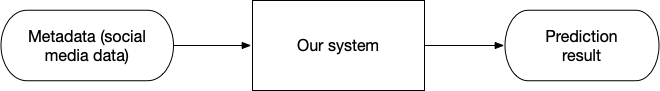
\includegraphics[width=5in]{images/system1.png}
    \caption{Blackbox}
    \label{fig:sys1}
\end{figure}
\\The aims of overall design involve building a complete process where the performance is reproducible, the subprocesses can be adjusted and the outcome can be easily understood and visualized. Based on it, we separate the Blackbox into 6 independent components: Data Collector, Preprocessor, Classification Model, Clustering Model, Evaluation layer, visualization. The overall structure can be seen in Figure \ref{fig:sys2}, the square represents component while ellipse represents data.
\begin{figure}[!htp]
    \center
    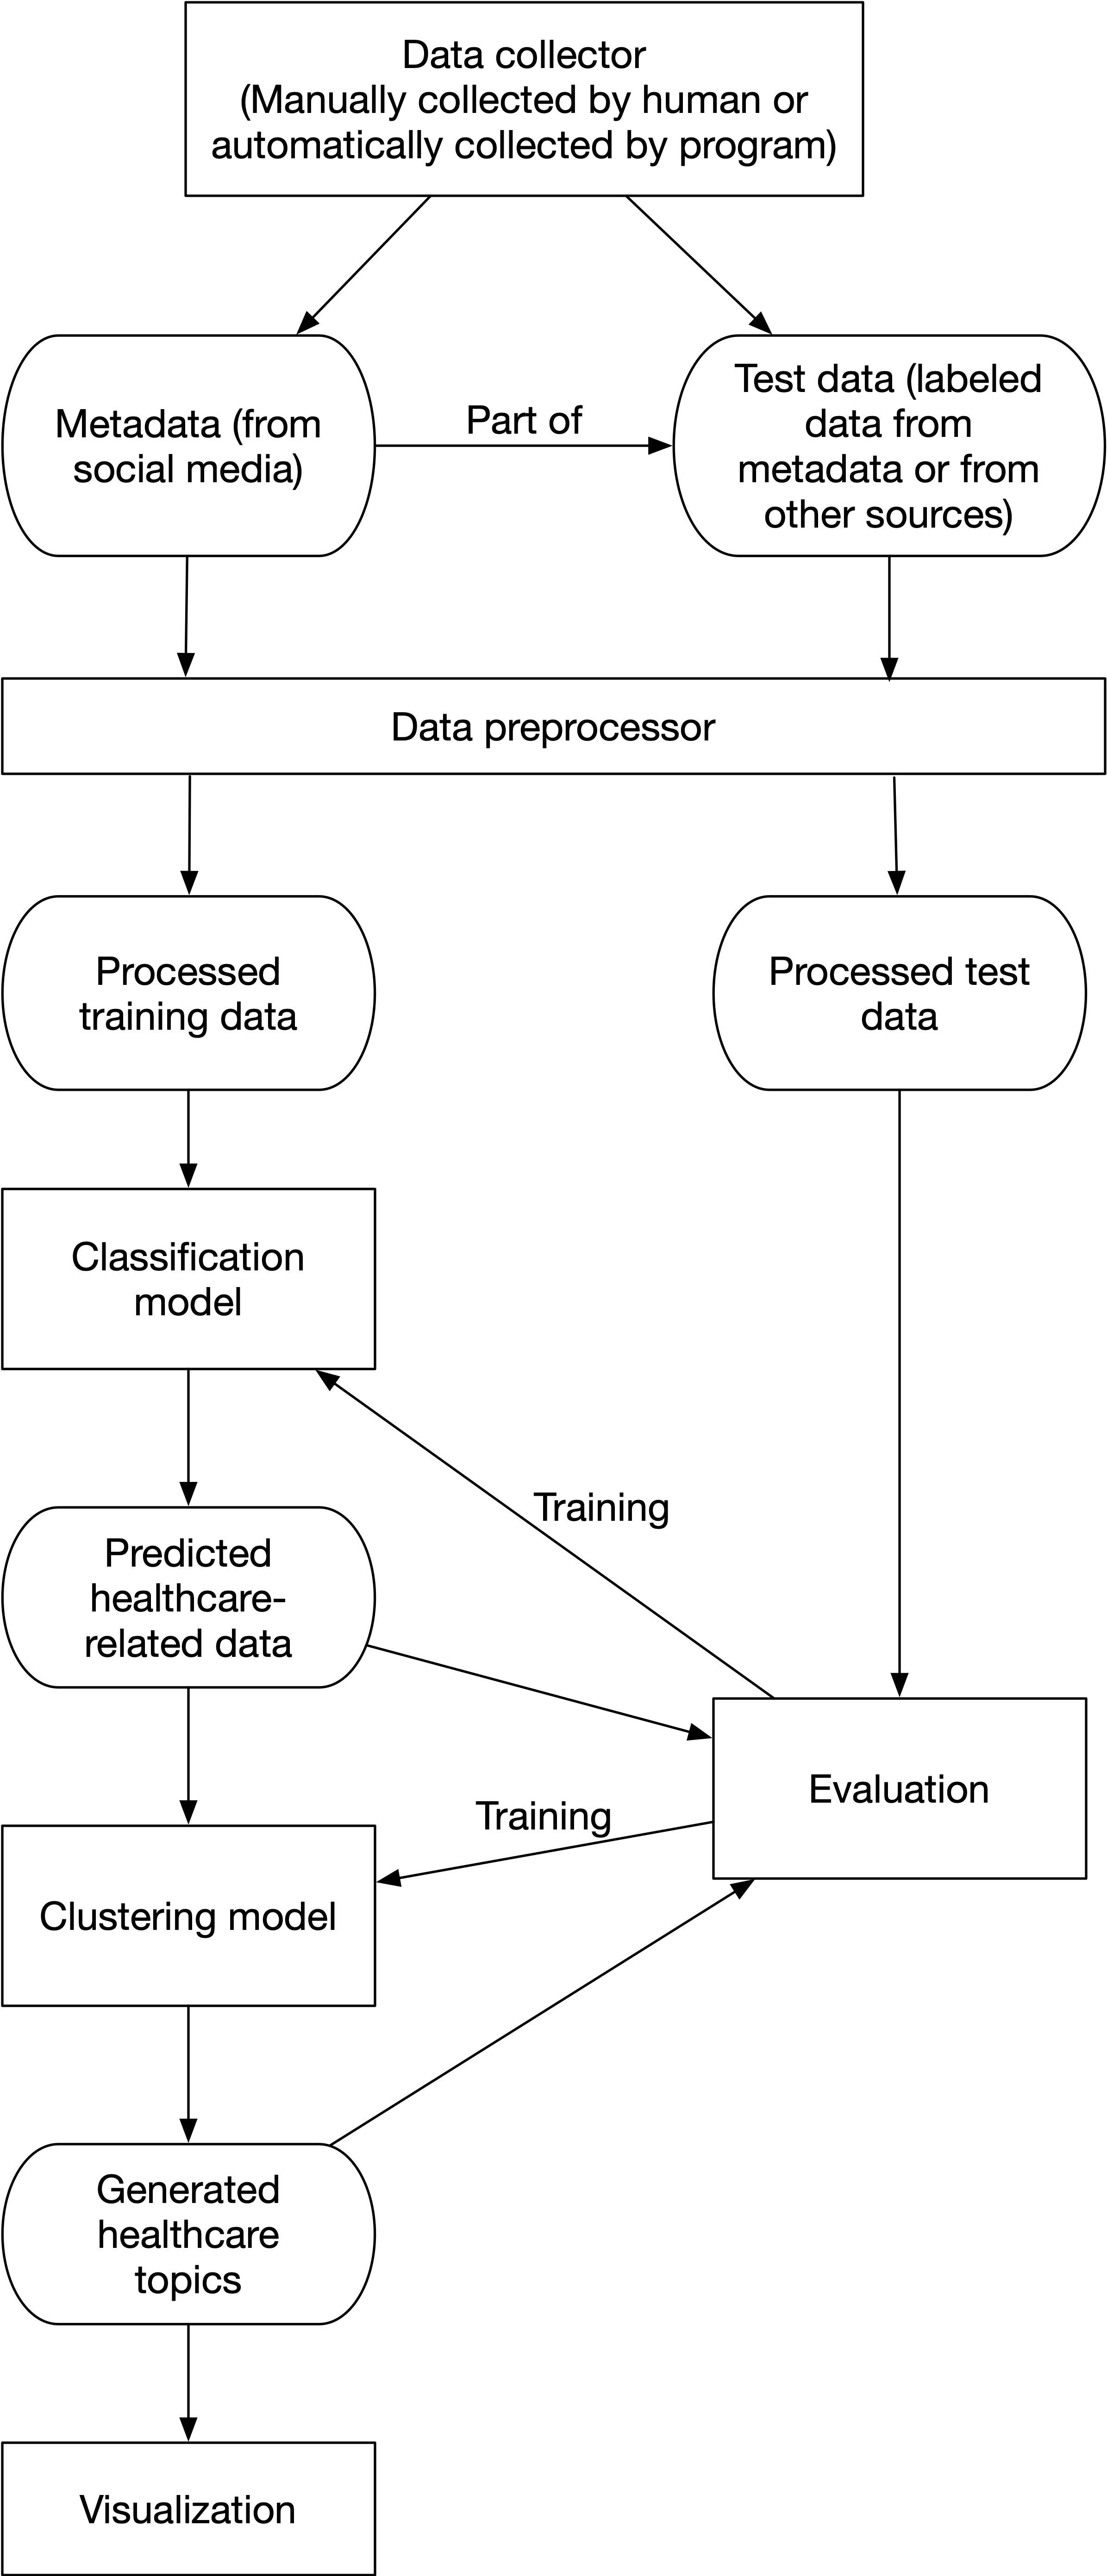
\includegraphics[width=3in]{sys2.jpg}
    \caption{Overall design}
    \label{fig:sys2}
\end{figure}
\section{Basic components}
This section show the preliminary design of our components, including the basic functional requirements of each part and the possible methods we may adopt. Following subsections represent stages(pipelines) of our system respectively, the general procedure design is inspired by \cite{feldman2007text}.
\subsection{Data collector design}
\label{sec:Data collector design}
Social media data is the input of the whole system, but according to the different social media platforms and various sources of data (such as extracted from official API or download from open-source dataset), the structure of data and methods of collecting data can be diverse. Therefore, we design an interface which can collect and integrate different metadata. In this project, we focus more on modeling and algorithm design rather than a complete system, therefore, we choose one certain social media platform. In addition, to evaluate the accuracy and performance of our model, we need a ground truth dataset (if available). Here the interface should at least collect these two dataset from at least one source respectively.\\
Functional requirements of this component are:
\begin{enumerate}
    \item Collect and store social media data from at least one source
    \item Collect and store ground truth data from at least one source, or manually label some data from metadata
\end{enumerate}
\subsection{Data preprocessor design}
\label{sec:Data preprocessor design}
Data collected by stage 1 are metadata, which could be unstructured and irrelevant to this project. We subdivide this step into smaller steps:
\begin{enumerate}
    \item Unify data structure: if one dataset comes from different sources (for example, facebook data extracted from API and from web spider). To pass these data into functions of later steps, a unified format is required. In addition, dataset could contain information that won't be used by our algorithm, ignore such information when unify data can save storage space. In our design, both unified structures of social media dataset and ground truth dataset should be implemented (see section \ref{sec:Data collection}). 
    \item Text regularization: social media dataset could adopt different coded format (such as ASCII and unicode), here we decide to use utf-8 encoding, which is wildly used in the Internet. The collected data could contain special symbols, unknown characters, URL links and emoji, pictures, videos (See Figure \ref{fig:tsc1}). In this project, we focus on pure text, thus information such as URL links, pictures and videos will be ignored. Inspired by \cite{serban2019real}, emoji and some pecial symbols can be transformed in to text based on standard transformation tables. We will adopt such transformation to keep maximum valuable data.
    \begin{figure}[!htp]
        \center
        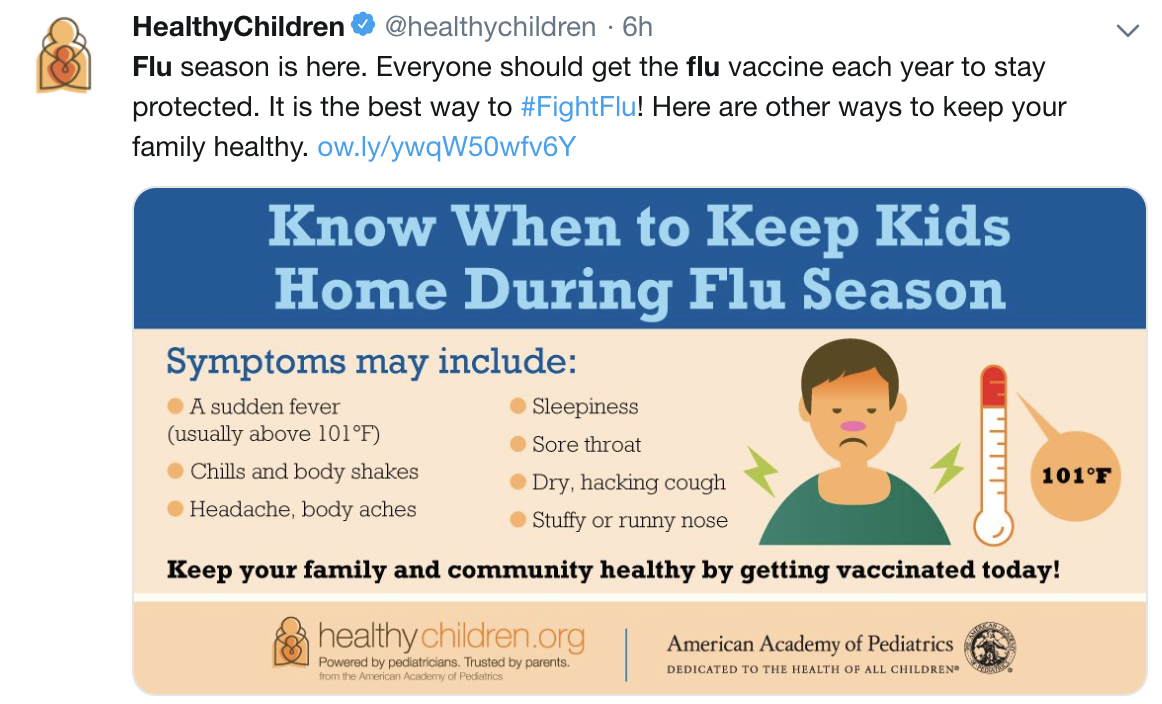
\includegraphics[width=4in]{images/tsc1.png}
        \caption{Tweet with URL and picture (screenshot from \href{https://twitter.com/search?q=flu&src=typed_query}{Twitter})}
        \label{fig:tsc1}
    \end{figure}
    \item Data filtering (classification): after the structuralization, the dataset can be used for analysis. However, not all the data contain information we want. This step will filter out irrelevant data of both social media dataset and ground truth dataset and reserve data that be considered useful. We will set inclusion rules and classifier to filter the data and label them (see section \ref{sec:Preprocessing}). The method we adopt to train a classifier is similar to how we build our prediction model. The detailed methods of text tokenization,encoding and building neural network model can be found in stage 3 of this section.
    \item Location extraction (possibly): in this project, we need data containing time of creation, geographic information to create our diffusion model. Data without such information can be used to train a classifier in the next step. The time of creation is contained in most sources (all the datasets we search so far provide temporal information). However, based on user's setting, some data don't contain geographic information (users can hide their private information if they wish). In addition, some platforms allow users name their own location (such as Wechat, users can assign personalized name to their location), or use a fake one. Platforms can adopt different standards of placename. Apart from that, even a user provide authentic private location, it still can't be guaranteed that he was in that place when posted tweets. All of such conditions bring noises in the dataset. Use the method we deal with unstructured metadata as reference, here we plan to the same solution: regularize the geographic information, set a standard in our project. In term of customized placename, we will design a function trying to map it to our standard (see Chapter 4). However, it worth noting that, the percent of social media with geographic information is comparably samll, which may not be sufficient to build a reliable predictive model (and this design could be changed based on it).
\end{enumerate}
Functional requirements of this component are:
\begin{enumerate}
    \item Must unify a data structure of social media dataset, and can integrate datasets (if more than one sources) into the same structure
    \item Must unify a data structure of ground truth datasets, and can integrate datasets (if more than one sources) into the same structure
    \item Must regularize all the text in the integrated dataset
    \item Must extract geographic information of each data if available
    \item Must regularize all the extracted geographic information into a unified format
\end{enumerate}
\subsection{Classification Model design}
\label{sec:First round predictor design}
As can be seen in figure \ref{fig:sys2}, the final model is designed as an ensemble of two models: a classification model and a clustering model. Classification model is help to screen out data that is irrelevant to healthcare, and hence we will use labeled data to fed it. Therefore, the model follows the the common process of solving NLP tasks.
\begin{enumerate}
    \item Text tokenization: neural network can only receive tensors as input, therefore, the first step of this stage is transforming the textual data into tensor, which is called tokenization (a token is a single unit extracted from text) \cite{Chollet:2017:DLP:3203489}. There are three basic word separation strategies: (1)split text into single words, transform each word into a vector; (2)split text into single character, transform each character into a vector; (3) extract n-gram of words or characters, transform each n-gram into a vector (a n-gram is a set of sequential words or characters), the resulting set is called bag-of-words \cite{Chollet:2017:DLP:3203489}. Bag-of-words can't record the order of words in the original text, therefore, this method is wildly used in shallow-layer model instead of deep learning model. Extracting n-gram is a feature engineering, which is inflexible and unstable. Here we adopt the first strategy, the feature extraction procedure will done by our deep learning model.
    \item Text encoding: the procedure that transform token into vector is called encoding. There are two most common methods. One is one-hot encoding, which assign each token a unique integer i, transform i into a binary vector (only contains 1 and 0) of length N (N is the size of token list), only the ith element is 1, others are 0. This method returns a high dimensional sparse vector (20000 dimensions or more), since each token takes one dimension. Anthoer encoding method is word embedding, which is learnt from dataset, returns a low dimensional intensive vector. The idea behind this method is that: the geometrical distance of two token should base on their relation (synonyms should have shorter distance than antonyms), and the vector's direction should have sense. For example, the vector of word ``king'' plus the vector of word ``female'' should return the vector of word ``queen'' \cite{Chollet:2017:DLP:3203489}. Therefore, we can't assign each token a vector randomly. In addition, for different tasks, the embedding space could be diverse, the embedding space used for sentiment analysis may not fit argot detection. In our design, we will try both of these two methods, and for the second, we will train a embedding space based on our dataset.
\end{enumerate}
\subsection{Clustering model design}
Some topics could be relatively new or have few samples, it's hard to label the classes of them in advance. Therefore, the classification model could not predict all minor topics related to healthcare. For this reason, we decide to use one more unsupervised model that helps to detect health events. Classification is in charge of deciding whether a given document contains information about healthcare, while the clustering model groups the filtered data in a time slice (such as in one day) and find the hidden topics. The functional requirements of this model are:
\begin{enumerate}
    \item Must take the filtered data from the classification model, and group them into clusters
    \item Must assign a interpretable topic to each cluster
\end{enumerate}

\subsection{Evaluation layer design}
\label{sec:evaluation}
In our overall design (Figure \ref{fig:sys2}), there are two cycles linking this layer and two models respectively. This doesn't mean that those two model share the same evaluation criteria. In deed, this layer is abstract, it is designed to show that we will evaluate this two models respectively. 
\\\\For the supervised classification model, according to \cite{Chollet:2017:DLP:3203489}, there are 8 common methods can be adopted to evaluate the model: (1) confusion matrix; (2) accuracy; (3) precision; (4) recall; (5) F1 score; (6) ROC curve; (7) AUC (Area Under Curve); (8) PR curve. Especially, accuracy and recall are wildly used in class-imbalance problem (our task is class-imbalanced). Following are formulas of (2)(3)(4)(5), where TP, TN, FP, FN represents true positive (the number of cases correctly identified as required), ture negative the number of cases correctly identified as not required, false positive (the number of cases incorrectly identified as required), false negative (the number of cases incorrectly identified as not required), respectively:
\begin{displaymath}
    \begin{array}{c}
        Accuracy = \frac{TP+TN}{TP+FN+FP+TN} \\
        Precision = \frac{TP}{TP+FP}\\
        Recall = \frac{TP}{TP+FN}\\
        F1 = 2\times\frac{Precision \times Recall}{Precision + Recall}
    \end{array}
\end{displaymath}
Once the socre (target) is defined, we must adopt a method to assess the result. There are 3 common methods: (1) Hold-out method (test set estimation); (2) K-Fold Cross Validation; (3) Repeated k-fold Validation. The first method works by randomly divided dataset into two mutually exclusive subsets, the training set (often $\frac{2}{3} to \frac{4}{5}$ of the original set) and testing set. It is simple to implement but will be severely affected by the size of subsets. If the training instances is far more than testing instances, the evaluation result is unreliable, but in reverse, the model will lose fidelity. In addition, this method is unsuited to small sample sizes, since it can't make full use of data\cite{omary2010machine,Chollet:2017:DLP:3203489}. Second method partition data into k separate subsets of similar size. Each subset will be used as testing data in turns (k times) while left subsets will be used as training data, the final socre is the mean of all rounds. It can be regarded as a kind of hold-out method with the ability to exploit more data and provide higher reliability \cite{omary2010machine}. The third one is used when the available data are too fewer while high prediction accuracy is required. It repeat the second method and calculate average score \cite{Chollet:2017:DLP:3203489}.  \\
\\For the clustering model, there are several criteria, such as Silhouette Coefficient. However, we care more about the interpretability of generated topics rather than the grouped clusters. Here we decide to use coherence of topics to evaluate our model. The details can be found in section \ref{sec:unsupervised}.
Functional requirements of this component are:
\begin{enumerate}
    \item It should provide different evaluation indexes (Accuracy, Recall, etc.)to assess the prediction outcome.
    \item It should provide different evaluation methods (K-Fold, Hold-our, etc.) to assess the prediction outcome.
    \item Must choose a best combination of methods to evaluate prediction result based on ground truth dataset.
    \item Must set a baseline (or target) to stop training.
    \item The evaluation result must correlate with human judgement.
\end{enumerate}
\subsection{Visualization design}
The final result may not clear and meanful for users. Visualization can help users/researchers to figure out the potential information of data/result, such as its feature, pattern, trend and relationship \cite{grinstein2002information}. There are various visualization techniques for different sceniros, purposes and data/input, such as 2D display (bar chart) and 3D display (cloud vapor), in addition, if the prediction is real-time, the visualization could be dynamic.  In this project, visualization is used in the last stage, therefore, we can assume the the input is stable and predictable. In addition, the prediction is numerical, according to \cite{grinstein2002information}, geometric representing methods could be used, such as scatetr plot, lines etc. The final method will be adopted based on the experimental result.\\\\
Functional requirements of this component includes:
\begin{enumerate}
    \item It should integrate the whole process and choose an approach to display the result.
\end{enumerate}

\chapter{Data collection and processing}
In our system design, there are two general datasets are needed. The first is the social media textual data, which is the most vital to this system, called social media dataset. It contains the implication of potential outbreak of diseases, all the prediction are made based on it. However, to evaluate the accuracy of the prediction, actual records of diseases are needed to serve as benchmark. 
\section{Social media dataset}
\label{sec:Social media dataset}
In this project, we choose one certain social media platform to test our algorithm, that is the Twitter. More specifically, we focus on tweets expressed in English. These choices based on the characteristics of Twitter:
\begin{itemize}
    \item Providing location: In our design, the posting location of each post is required. And we found that Twitter provides such information. According to research conducted by \cite{greenwood2016social} in 2016, about 1.6 percent of Twitter users opted in Twitter's location-sharing service.
    \item Availability: Most tweets are available for research. According to \cite{serban2019real}, around 95\% of Twitter users opted in sharing their tweets with public, meaning their tweets can be searched and filtered by keywords without their permission.  
    \item Comparability: In our research, we found that most related works used data from Twitter, which means that Twitter dataset can act as a benchmark to evaluate our algorithm.
    \item Timely: According to \cite{serban2019real}, each tweet is received within seconds of their creation.
    \item High user volume: According to \cite{greenwood2016social}, about 21\% of American citizens use Twitter.
\end{itemize} 

\section{Benchmark}
In this project, we focus on one certain disease, flu. The benchmark used in this project is Fluview \cite{cdc:fluView}, a weekly-update, influenza surveillance report of the U.S. published by Centers for Disease Control and Prevention (CDC)\cite{cdc.gov}. Such report is a collaborative effort between CDC and its many partners in state, local, and territorial health departments, public health and clinical laboratories, vital statistics offices, healthcare providers, clinics, and emergency departments \cite{cdc.gov}. CDC maintains a surveillance network called Influenza-like Illness Surveillance Network (ILINet), which collect information on outpatient visits to health care providers for influenza-like illness \cite{cdc.gov}. We choose CDC's Fluview as our benchmark because of its:
\begin{itemize}
    \item Reliability: ILINet collects data from about 2600 outpatient healthcare providers across the U.S. weekly \cite{cdc.gov}.
    \item Accessibility: All the reports of Influenza-like Illness (ILI) can be accessed by public.
    \item Comparability: The dataset maps the activity of ILI into levels between 1 to 10, which can be used as labels or targets of our training data.
\end{itemize}
\begin{figure}[!htbp]
   \center
   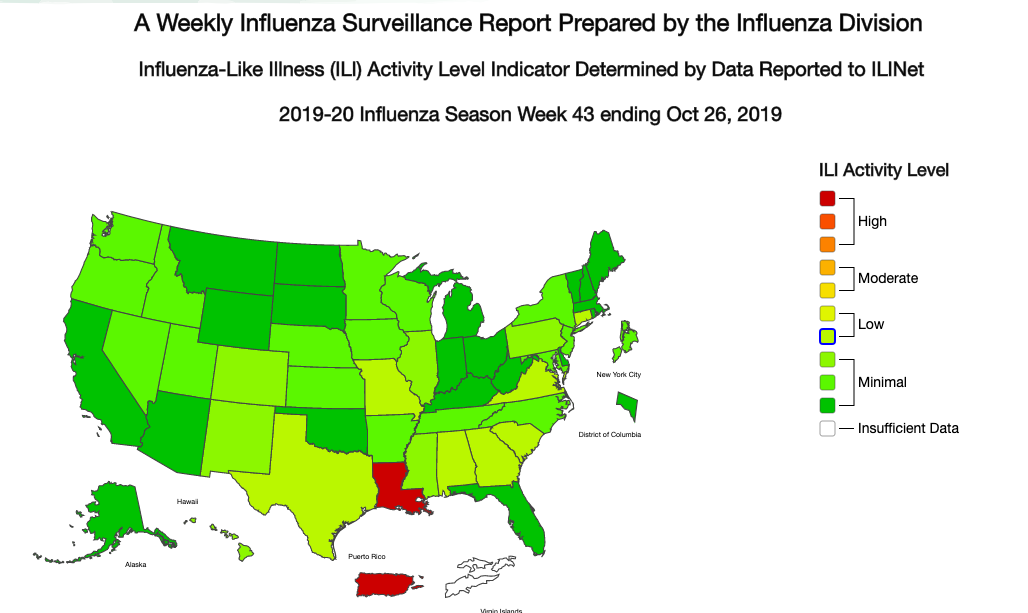
\includegraphics[width=6in]{images/week43.png}
   \caption{Influenza Season Week 43 ending Oct 26, 2019, Source: \href{https://www.cdc.gov/flu/weekly/index.htm\#ILIActivityMap}{Fluview}}
   \label{fig:fluView}
\end{figure}
Figure\ref{fig:fluView} shows the ILI activity levels across the U.S. in Week 43, 2019. It can be seen that the there are 10 levels divided into 3 categories, each level is assigned a unique color.
\section{Data collection}
\label{sec:Data collection}
This section shows the detailed methods of how we collect data and unify the data structure. 
\subsection{Twitter dataset collection}
\label{sec:Twitter dataset}
In this project, we collect Twitter data from Internet Archive\cite{archive}, a non-profit digital library of millions of free books, movies, software, music, websites. It contains daily tweets from Feb 2011 to Jul 2019 (Accessed: Dec 08,2019). All the data are Spritzer version (roughly 1\% of the whole tweets) grabbed from the general twitter stream The number of tweets collected in Oct 05 2018 is 4273031, in Oct 04 2018 is 4337327, in Oct 01 2018 is 4317376, on average is above 4 million per day. All the tweets are stored in json files. Such data volume is sufficient for our research and its data structure is convenient to use. More important, it contains the information we need, which mentioned in section \ref{sec:Social media dataset}. Figure \ref{fig:archive1} shows part of the information those json files contain (geographic and linguistic information are contained but not listed here). In our project, we mainly focus on tweets posted during 2018.\\
\begin{figure}[!htbp]
    \center
    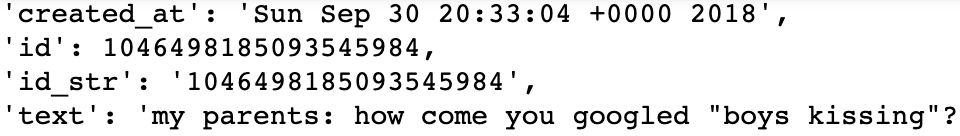
\includegraphics[width=5.5in]{images/archive1.png}
    \caption{Screenshot of Archive's Twitter data}
    \label{fig:archive1}
\end{figure} 

\subsection{Fluview dataset collection}
This data can be downloaded from official websites of Fluview \cite{cdc:fluView} (Accessed: Dec 08,2019), user can customize the data they want to download (the time span of reports). All the information is stored in a single csv file. Figure \ref{fig:fluView1} shows the structure of the data. 
\begin{figure}[!htbp]
    \center
    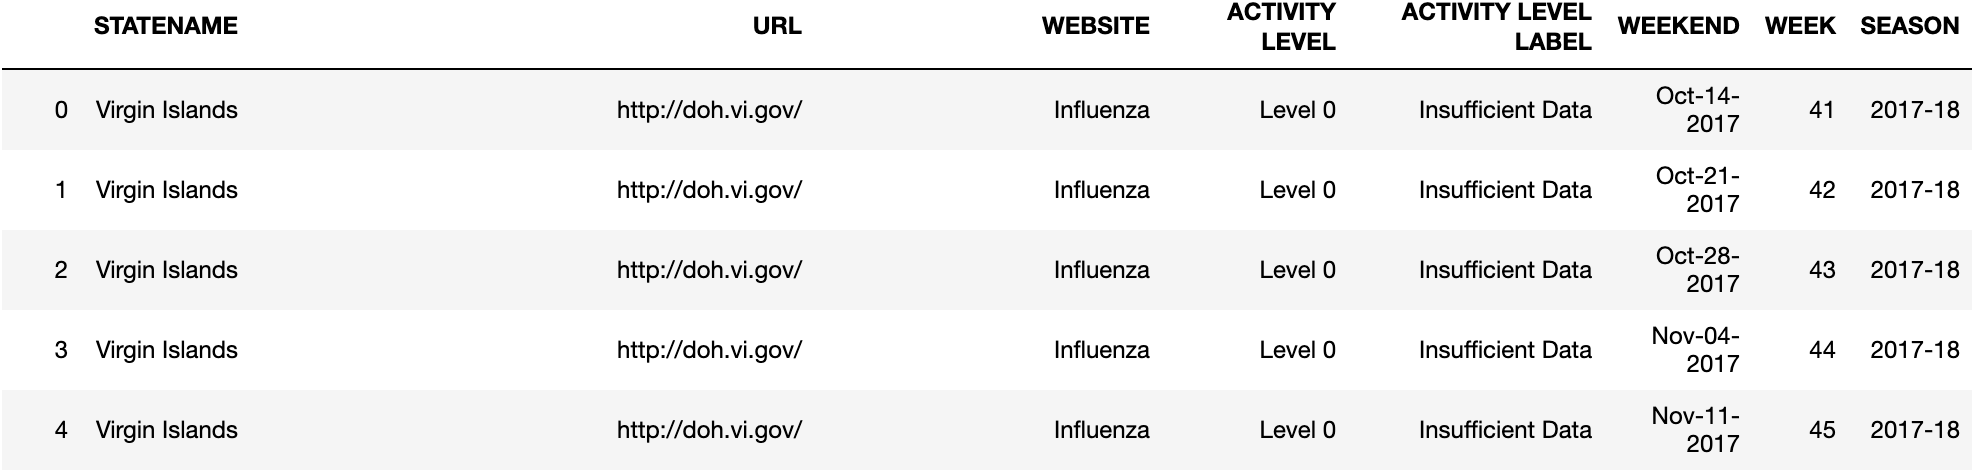
\includegraphics[width=5.5in]{images/fluView1.png}
    \caption{Screenshot of Fluview's report}
    \label{fig:fluView1}
\end{figure}
\\
Our data structure is a cut-down version of it, where ``URL'' and ``WEBSITE'' columns are deleted. ``WEEKEND'' is transformed into the format we used in Twitter dataset.

\section{Data Preprocessing}
\label{sec:Preprocessing}
Data preprocessing is the first stage of a typical text classification framework. According to experiment conducted by \cite{uysal2014impact}, different combination of preprocessing methods can influence the accuracy of prediction. However, there is no best combination for all tasks. Some strategies can improve classification success of certain tasks while lower that of others.
\begin{figure}[!htbp]
    \centering
    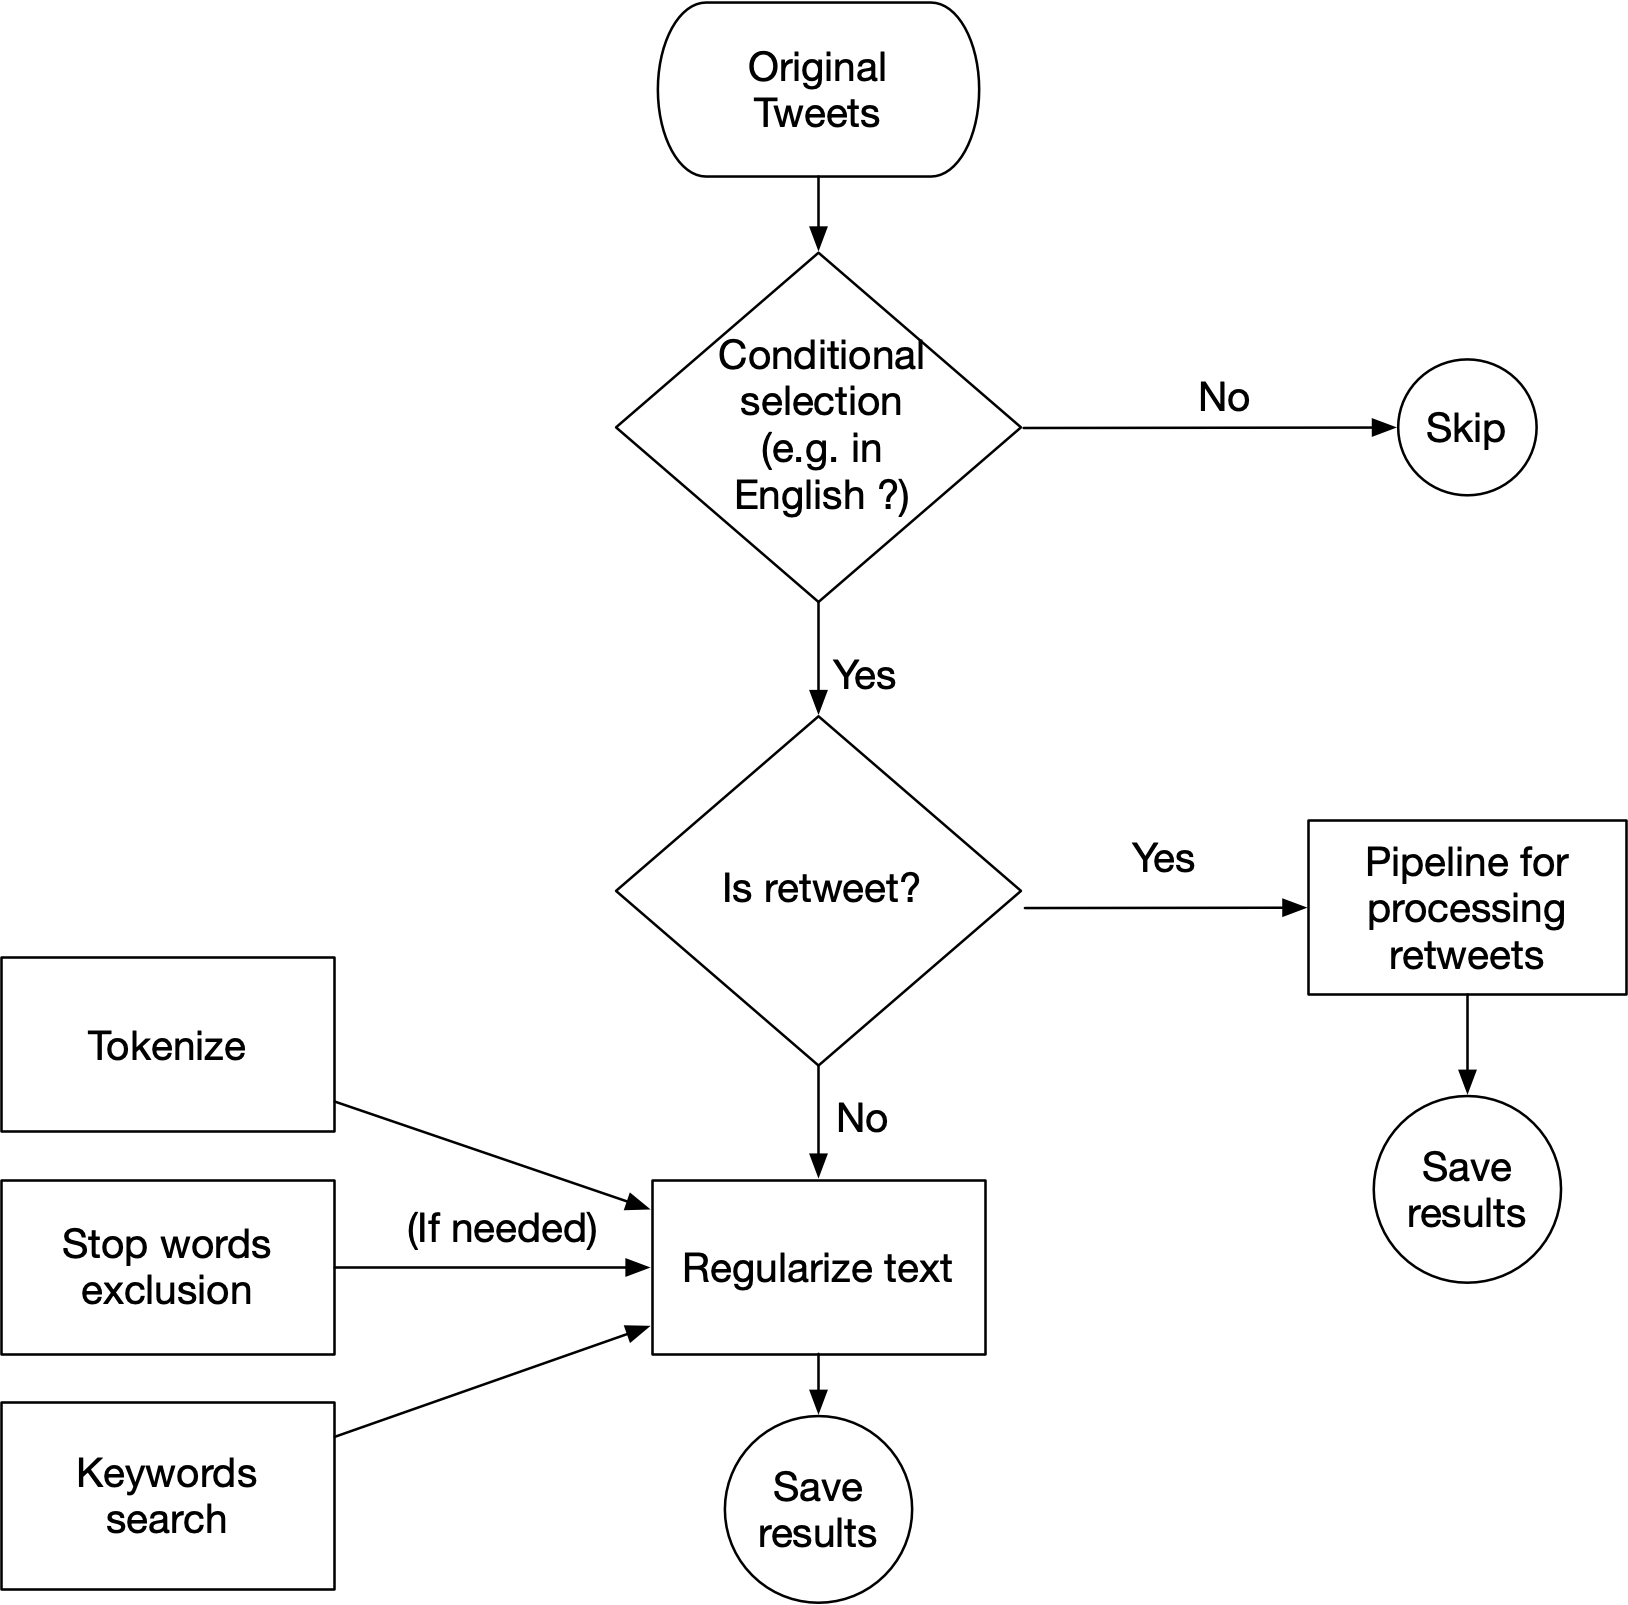
\includegraphics[height=3in]{pipeline.jpg}
    \caption{Common pipeline of text preprocessing}
    \label{fig:pipeline}
\end{figure} 
Figure \ref{fig:pipeline} shows some common steps used in NLP for preprocessing textual data. Following sections represent our preprocessing methods designed for this project.
\subsection{Unify data structure}
\label{sec:Unify data structure}
In section \ref{sec:Data collector design}, we mentioned a unified data structure of our datasets. The aim of this stage is to unify and regularize all the metadata before analysis. \\
\\The Fluview dataset is well structured (see Figure \ref{fig:fluView1}), and can be used in our system directly (we used its ``STATENAME", ``ACTIVITY LEVEL", ``ACTIVITY LEVEL LABEL'' and ``WEEK'' columns). One point should be noticed here is that the STATENAME used in Fluview dataset can be different from that in Twitter (Twitter' users can set their own location), therefore, we created a unified name list of states and a function designed to regularize different geographic information.\\
\\
Our social media dataset's structure is built on Twitter's official data structure \cite{twitter_dev}, and we only reserve the information we may use. It is a hashmap with 5 keys: ``created\_at'', ``text'', ``location'' and ``coordinates'', ``place''. We regularize the time into format Year/Month/Day (2018/10/01) and store it in ``created\_at'' keys, exclude other information (see Figure \ref{fig:social_data_sture}). Note that in the metadata, there are massive ``deleted'' tweets, which contain no textual information, and we removed all such data.
\begin{figure}[!bp]
    \centering
    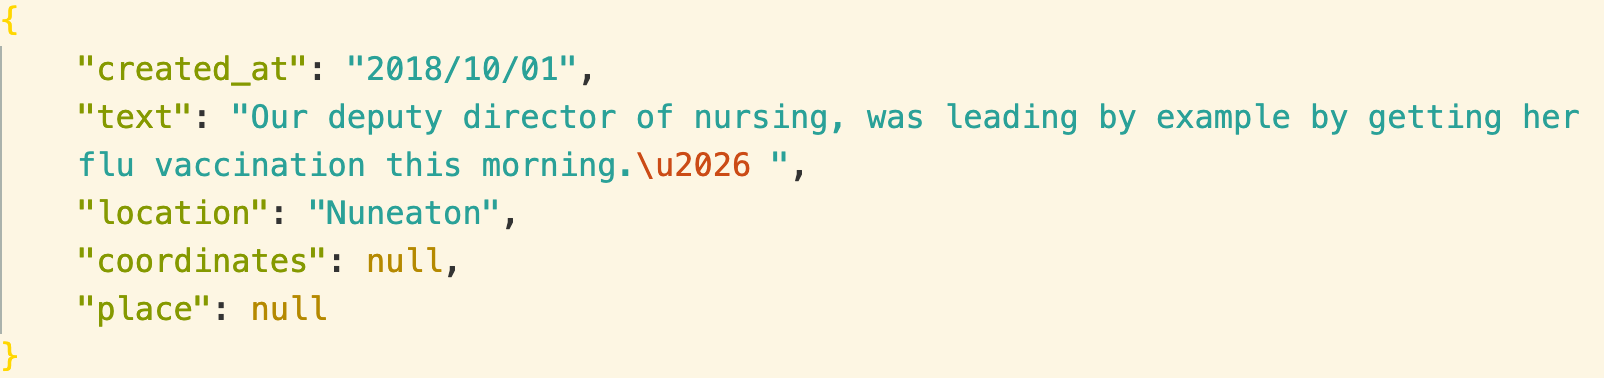
\includegraphics[width=5in]{images/dataset1.png}
    \caption{Screenshot of unified structure of social media dataset}
    \label{fig:social_data_sture}
\end{figure}
According twitter's official document \cite{twitter_dev}, there are two classes of geographical metadata in Tweet data: (1) Tweet location, which is available when users share location at time of Tweet; (2) Account Location: a free-form character field set in user's profile and may or may not contain metadata that can be geo-referenced. ``location'' attribute stores the user-defined placename. ``coordinates'' attribute provides the exact location of a tweet (in long-lat order) but has no placename and only available when the location is assigned. ``place'' attribute is always present when a Tweet is geo-tagged, and it contains Twitter ``place'' with a display name and type. Here we keep all these three keys, and ``place'' key gets the first priority when we extract location of tweet. Figure \ref{fig:twitter_place} shows a sample of Twitter ``place''. Note that most data don't contain ``location'', ``coordinates'' and ``place'' keys, which is expected in section \ref{sec:Social media dataset}.
\begin{figure}[!htbp]
    \centering
    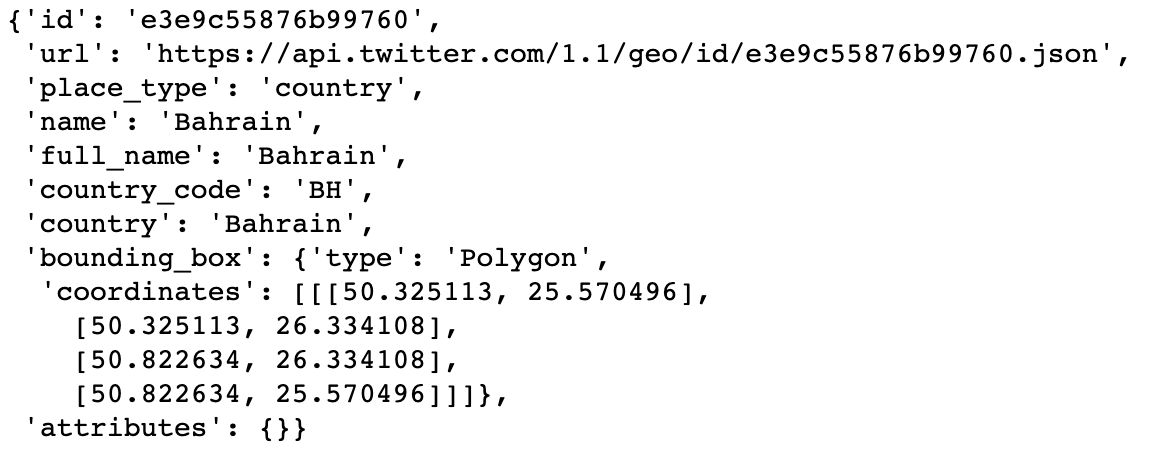
\includegraphics[width=5in]{images/twitter_place.png}
    \caption{Screenshot of Twitter's place object from our dataset}
    \label{fig:twitter_place}
\end{figure}

\subsection{Text regularization}
As mentioned in our design (section 3.2.2), the original text is unstructured, which can not be put in to our model directly and hard for labeling. In addition, each dataset has its own structure, meaning that there is no common regularization rule can be applied to all tasks. Here our regularization rule is built on the observation of our dataset and on our experience. Followings are common formats we observed and removed (or modified) in our dataset, expressed in regular expression (Python version):
    \begin{itemize}
        \item retweet: retweeting is a way of forwarding content to others (like forwarding an email). It starts with a ``RT \@'' pattern. As we mentioned in section \ref{sec:Manually screening}, we removed all retweets.
        \item @ and \# Tags: in social media, @ refers to a person/group in a conversation, and the \# refers to a topic of conversation. Their regular expression are ``\@+[\verb|\|S]*'' and ``\#+[\verb|\|S]*'' respectively. In our preliminary filtered dataset, we found that some topics contain words in our inclusion list, such as \#ALDUBFever4ever. We exclude them. 
        \item URL links: some tweets contain URL links starting with ``http'', ``ftp'' or ``https'', which can't contribute to our classification. Its regular expression is:\\``http[s]?://(?:[a-zA-Z]$|$[0-9]$|$[\$-\_@.\&+]$|$[!*\verb|\|(\verb|\|),]$|$(?:\%[0-9a-fA-F][0-9a-fA-F]))+''
        \item emoji: emojis in our dataset are encoded in unicode, inspired by \cite{serban2019real}, some of them can be translated into their name based on emoticon dictionaries. Through our search, we find a Python library called \href{https://pypi.org/project/emoji/} {emoji(version 0.5.4}), which embedded the full emoji list from \cite{emo_list} and can help us to translate emoji into text through function call \cite{pytho_emo}. Figue \ref{fig:emo_lib} shows a example how to use this library, the translated emojis are embraced by `:' signs by default. In our implementation, each translated emoji is assigned a prefix `emo\_' to identify it, and we separate emojis with a blank space for split convenience.
        \begin{figure}[!htbp]
            \centering
            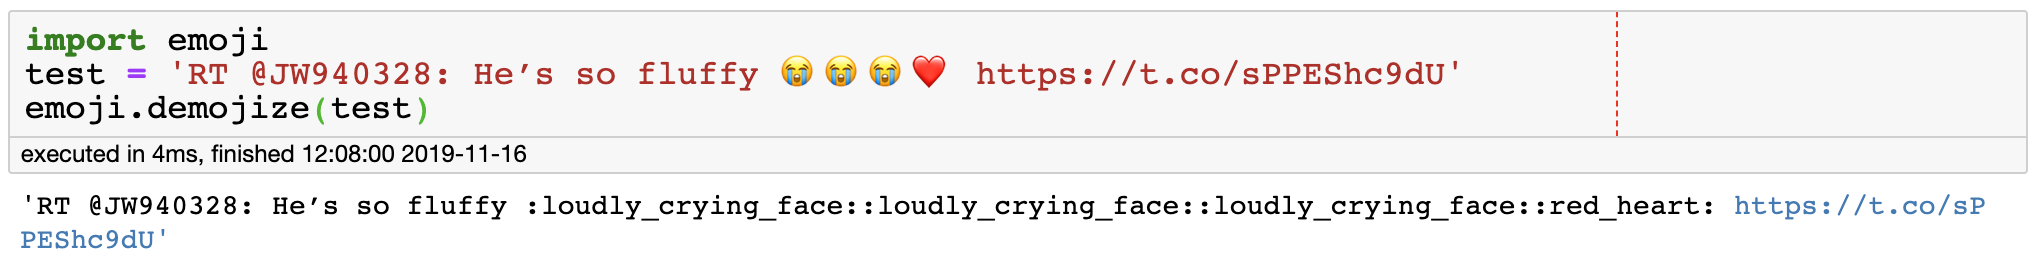
\includegraphics[width=5in]{images/emoji_lib.png}
            \caption{Example of using emoji library}
            \label{fig:emo_lib}
        \end{figure}
        \item e-mail address: we exclude e-mail address in our data, whose regex(can match most e-mail addresses) is:
        ``[a-zA-Z0-9\_.+-]+\@[a-zA-Z0-9-]+\verb|\|.[a-zA-Z0-9-.]+\$''
        \item html entities: a html entity can be regarded as escape characters used in html (eg. \&quot; represents ``'' sign). We use the Python's standard library ``html'' to translate it.
        \item non-Latin characters: characters that are not in Latin are meaningless, we exclude them with regex ``[\^A-Za-z0-9\_]'' 
    \end{itemize}
    In addition, for next steps, all the text are in lower case.

\subsection{Manually screening}
\label{sec:Manually screening}
We have more than 4 million tweets per day in our dataset, it's obviously not all of them are relevant to our task. Based on our initial design, we only accept tweets written in English. While reviewing on the dataset, we found that there are massive retweets in it (8312846 of 21694196, roughly 38\%). Defined by Twitter\cite{twitter_dev}, retweeting is forwarding content wrote by other users (like forwarding an email). Although retweets can be used in some tasks such as sentiment analysis (mainly focus the counts of being retweeted) \cite{perdana2018combining}, we don't think it will contribute to our prediction. As stated by \cite{kim2016competitive}, retweets don't have user's own view and should be removed in data cleaning. We need tweets that can show the health condition of the user or of people the user cares. In addition, retweets don't have any geographical information \cite{twitter_dev}, which is the key component in our diffusion modeling. Therefore, we decided to exclude all retweets.\\ Furthermore, we exclude all non-English tweets by the tag contained in metadata. Table \ref{tab:manual} shows the result of manually screening operated on all tweets created at January 2018 in our metadata. Original data amount is 134704400, nearly 13.87\% are retweets, and 23.40\% are English. After screening, roughly 10.22\% tweets were left.
\begin{table}[!htbp]
    \centering
    \hspace{0.5cm}
    \begin{tabular}{cccc}
        Original & Filtered & Retweets & English\\ \hline
        134704400 & 13643710 & 18682273 & 32325983
    \end{tabular}
    \caption{Result of Manually filtering}
    \label{tab:manual}
\end{table}
\\
Since Twitter dataset contains massive tweets which are irrelevant to flu, before we analyze the data, further filtration is required. We adopt two steps to filter out irrelevant data, keywords search and supervised classification. Following sections are the details of these two methods.

\subsection{Keywords search}
\label{sec:Keywords search}
To filter out irrelevant data, \cite{aramaki2011twitter} used a simple word look-up of ``influenza'',which we think may lose massive valuable data. In inspired by \cite{lamb2013separating,lampos2010flu}, we first create a word list related to flu based on Flu Symptoms \cite{cdc.symp} Cambridge Dictionary \cite{cambridge} and relatedwords.org \cite{relatedwords.org}. The complete word list can be seen in table \ref{tab:words list}, note that not all the words from the sources are added to our list. Professional terms are excluded since they are hardly used in colloquialism. Words that are wildly used in other scenarios (such as chill, cold) and phrases that contain keywords in our list (such as asian influenza) are not added. We then filter tweets according to the list (ignore case). In this step, we initially adopted a relatively lose filtering strategy: accept tweets containing any string in our list. 
\begin{table}[!htbp]
    \centering
    \hspace{0.5cm}
    \begin{tabular}{p{90pt}p{320pt}}
        Source & Word list \\ \hline
        \href{https://www.cdc.gov/flu/symptoms/symptoms.htm}{CDC} &  fever, feverish, sore throat, runny nose, stuffy nose, headache, nasal congestion, diarrhea, bluish lips, bluish face, dehydration\\ \hline
        \href{https://dictionary.cambridge.org/us/topics/disease-and-illness/colds-and-flu/}{Dictionary} & flu, catarrh, cough, common cold, influenza, sniffle, snuffle\\ \hline
        \href{https://relatedwords.org/relatedto/flu}{relatedwords.org} & h1n1, h5n1, coughing, cholera, ebola, epidemic, feverous, measles \\ \hline
    \end{tabular}
    \caption{Inclusion list}
    \label{tab:words list}
\end{table}
\\
Table \ref{tab:filtering} shows the number of tweets after keywords filtering in the first 5 days in Oct 2018 (retweets are included), and the filtered result operated on tweets created in Jan 2018 (without retweets). 
\begin{table}[!htbp]
    \centering
    \hspace{0.5cm}
    \begin{tabular}{ccc}
        Date & Original & Filtered \\ \hline
        2018/10/01 & 4317376 & 5984 \\
        2018/10/02 & 4349129 & 5740 \\
        2018/10/03 & 4417333 & 5415 \\
        2018/10/04 & 4337327 & 5676 \\
        2018/10/05 & 4273031 & 5190 \\
        2018/01 & 134704400 & 37519 \\
    \end{tabular}
    \caption{Tweet counts after filtering}
    \label{tab:filtering}
\end{table}
\\\\
We found that the majority of the filtered tweets are irrelevant to diseases. The possible reasons can be that people will use such words even when they are healthy, and some words are substring of other words (such as chill Achill, flu influence). Another probelm found after this step is that the volume of filtered data is less than our expectation. When retweets are included, nearly 0.129\% data are left. Exclude retweets, the percentage drops to 0.0279\% (although the experiment doesn't operate on a same sample). Note that in our initial design, we will use geo-tagged tweets (tweets with geographic information) created at certain regions, meaning that the percentage of our target data could be much lower (less than 0.01\%). Under such condition, we need massive data to get a reliable estimation (i.e. to get 10000 filtered data, at least 100000000 metadata are required). For research, it's impractical, and we decide to change the initial design.

\subsection{Supervised classification}
\label{sec:Supervised classification}
To overcome the drawbacks of first round filtration, further filtration is required. \cite{elkin2017network} created another exclusion dictionary containing keywords and phrases indicating tweets should not be included in the filtered dataset, such as "sick and tired". But their experiment shows the accuracy of their method is roughly 70\%, which we think is relatively lower than our requirement. This result can result from their choice of exclusion words and their dataset.  Since we want to get a higer filtering accuracy, we decide to use a machine learning based classification method \cite{aramaki2011twitter}. We labeled our dataset, and trained a binary classifier. Following are our detailed methods:
\begin{enumerate}
    \item Data labeling (classification): as mentioned before, we want to our classifier can tell wether a tweet is relevant to flu, therefore, we adopt a simple binary labeling strategy. We write a piece code and manually labeled the regularized data 1 and 0 (1 means it indeed relates to flu). While labeling, we found that some tweets can't be told wether they are truly related to flu, such as ``Coughing!'', ``i'm chilling'. And since in our first filtering (section \ref{sec:Keywords search}), we adopt a relatively loose rule, which accepts tweet that containing any string (word) in our inclusion dictionary, no matter the word is indeed a sub-string of another word (eg. flu and influence), the majority of filtered tweets (roughly 83\%, 450 of 540) are toally irrelevant to flu. In addition, some tweets are flu-related, but don't show signs of catching a flu, such as ``Just had my flu jab!''. All the problems mentioned above increase the difficulty of labeling. While we have more than a billion raw data, we decide to change our initial design and set a strict standard in filtering. Followings are our specific labeling rules: 
    \begin{itemize}
        \item tweets that don't contain any exact word in our word list will be excluded (eg. tweet containg ``feverfew'' and no other keywords won't be accepted even it has string ``fever'')
        \item tweets containing fewer words (no specific number) will be label 0, even they have our keywords insinde (eg. ``coughing!''), since they can hardly be classified
        \item tweets containing keywords but are irrelevant to flu will be labeled 0 (eg. ``Monday Chill. Always Chill'')
        \item tweets talking about flu outbreak happened in the history and past, about catching a flu before (months or years ago) and about flu statistics will be labeled 0 (eg. ``Over 80,000 Americans Died of Flu Last Winter, Highest Toll in Years'')
        \item tweets talking about flu but don't have signs of catching flu or outbreak of flu will be labeled 0 (eg. ``Flu vaccine is very safe - risk of serious reaction is less than one in a million, much lower risk than catching the flu'', ``It's that time of year again. Here are some tips to help your child get through a cough or cold.'')
        \item tweets containing symptoms of flu but can't tell the whether such symptoms are result of flu will be labeled 0 (eg. ``i’ve had a headache since yesterday and i wanna die'')
        \item tweets meeting the requirements above but still cause confusion when classification will be labeled 0 (eg. ``All iwanna do is cuddleand not cough every minute'')
        \item only tweets containing real information of getting flu and can easily be recognized will be labeled 1 (eg. ``Oh, is it colds and flu? Get well soon, and rest'')
    \end{itemize} 
    All the examples given above come from our dataset. Note that this standard is still not precise enough and can't guarantee all the data are correctly labeled, since the classification result highly depends on individuals who label the data. To minimize such difference brought by manual work, we built a exclusion list based on our deliberate review on the dataset during labeling, and labeled tweet containing word in the list 0.
    \item Stop words elimination: stop-words are words that are not regarded as keywords in text mining. Examples are: is, am, did, a, an, the, ect. Exclude stop-words can reduce the length of the text and dimensionality of term space\cite{vijayarani2015preprocessing}. There are four stop-word removal methods: (1) manually define the removal list; (2) Zipf' law based methods, which removes the most frequent and least frequent words; (3) Mutual information method (MI), a supervised method that can evaluate the discrimination power of a term for classification; (4) Term Based Random Sampling (TBRS), which is based on a term's importance \cite{jivani2011comparative}. 
\end{enumerate}

\section{Healthcare topics uncovering}
\label{sec:uncoverig}
Based on the experimental results shown in section \ref{sec:Keywords search}, we conclude that our metadata may contain insufficient tweets related to flu that can help us to built a reliable model. The reasons could be: (1) our keywords list is incomplete; (2) the metadata is collected randomly from all tweets, and contains few flu-related data coincidentally; (3) the sample we used in experimental contains few flu-related data coincidentally; (4) the data volume we examined is too samll and can't represents the general trending. 
Since the metadata contains more than billions of tweets, 
Topics related to healthcare surveillance are massive, and based on the experimental results shown in section \ref{sec:Keywords search}, we cannot guarantee the metadata contain enough tweets of topic chosen by us. Therefore, we decide to use topic model techniques to uncover some health related topics. 
Probabilistic latent semantic analysis (PLSA) \cite{hofmann1999probabilistic} and Latent Dirichlet Allocation (LDA) \cite{blei2003latent} are two well-known conventional algorithms of information retrieval, but their performance may decrease when running on short document such as tweets because of data sparsity probelm. Twitter-LDA model \cite{zhao2011comparing} is a relative new algorithm for solving this probelm. However, it requires a word distribution of users (tracking all tweets published by a single user). Our dataset mainly focus on text rather than users, meaning that we cannot run Twitter-LDA on our data. Therefore, we adopt the online version of Biterm Topic Model (BTM) \cite{yan2013biterm, cheng2014btm}, which models the word co-occurrence patterns and gets a better retrieval result than LDA and PLSA on short text. The original implementation can be found on \href{https://github.com/xiaohuiyan/OnlineBTM}{GitHub}. \\

To get meaningful words referring to an extracted topic, we exclude stop words listed by NLTK (The Natural Language Toolkit) \cite{journals/corr/cs-CL-0205028}.

\chapter{Signal extraction}
\label{sec:uncoverig}
There are massive topics related to healthcare and diseases and them expand everyday, it's impractical to list them all. \cite{tuarob2013discovering} defined health-related messages as follows: (1) either a message indicates explicitly the sick (or health problems) of the author; (2) or the message contains the author's worries about health problems (e.g. someone else falling ill, disease outbreak). To surveille diseases, we want to cluster messages(tweets) into different groups, find out what topics are concerned about. The aim of this section is to build a model (or a ensemble of different models) that can: (1) check wether a input document is related to health; (2) assign the checked document to one best match topic. If there is no topic match it, create a new one and assign the document to it (one similar example is hot event discovery). To achieve this, the model should be able to: (1) update the parameters over new input; (2) handle unseen input (such as new words, new topics, new meaning of a seen word, etc.). As far as we know, there is no such model.
\\\\
In the existing works, there are two types of models: supervised and unsupervised. \cite{serban2019real,aramaki2011twitter,lampos2010flu,chen2017disease} use supervised machine learning and deep learning techniques to detect flu. Their experimental results show that when used to detect the known disease, supervised models can get high accuracy. However, the performance of such model highly depends on the training set. For topics that are not in the training set, supervised models cannot recognize it. 
Hence a single end-to-end supervised model (label the data in advance) is not be qualified under this scenario. \cite{paul2012model} introduces Ailment Topic Aspect Model (ATAM) that amis to classify aliments. ATAM is an unsupervised model, requires a set of aliments and the prior distribution of them. Its essence is an variant of LDA, and the hyper-parameter K (the number of diseases/topics) is defined before training. Since the aliments and symptoms are pre-defined, ATAM cannot be treated as a pure unsupervised model, and it can't recognize new health event. However, pure unsupervised models cluster data based on its structure, and therefore are not able to identify whether a document is health-related or not. In addition, the generated topics are hard to interpret. Hence, to achieve the requirements of our model, both supervised and unsupervised methods are required.
\\\\
To extract health-related tweets and topics, \cite{paul2014discovering, paul2011you} described a general framework with 2 main phases: data filtering and topic modeling. The first phase is vital for narrowing down search space. They adopt keyword searching and machine learning as data filtering method. 269 keywords and 20,000 keyphrases were collected and used to filter out irrelevant data roughly. Then 5128 tweets selected randomly from dataset were labeled for training a SVM classifier that identifies wether a input is or isn't health-related. In the second phase, probabilistic topic modeling such as LDA and ATAM are used to cluster tweets and get interpretable topics. \cite{serban2019real,sadilek2012modeling} followed the same framework to classify tweets in their system, with some variance on data labeling, keywords list and classifier. \cite{elkin2017network} used exclusion list rather a classifier in phase one. 
\\\\
Before adopting any existing framework, we used Online Biterm Term Modeling (OBTM, a unsupervised Topic modeling algorithm, details can be found in section \ref{sec:topic modeling}) on a sample of processed data, to see how many health-related topics can be found. The sample covers all processed tweets created at Jan 2018 (13,643,710 non-retweet english tweets). The algorithm took three days on calculation to cluster documents into 100 topics. Merely few topics contain words related to health while they are hard to interpret. Similar experimental results can be found in \cite{zhao2011comparing}, where the authors calculate the distribution of topic categories, and find that roughly 5\% tweets are about health. To narrow down the search space, decrease the running time and make the final results more interpretable, our project adopts a similar framework with \cite{paul2014discovering}: use the keywords search first, then cluster topics. The details and experimental results are in following sections.

\section{Keywords search}
\label{sec:Keywords search}
Influenza is one of the most common diseases and is analyzed most by researchers. For scientific comparison, it was used to test the dataset. \cite{aramaki2011twitter} used a simple word look-up of ``influenza'', which may lose massive valuable data. In inspired by \cite{lamb2013separating,lampos2010flu}, we create a list with 26 words highly related to flu based on Flu Symptoms \cite{cdc.symp} Cambridge Dictionary \cite{cambridge} and relatedwords.org \cite{relatedwords.org}. The complete word list can be seen in table \ref{tab:words list}, note that not all the words from the sources are added to our list. Professional terms are excluded since they are hardly used in colloquialism. Words that are wildly used in other scenarios (such as chill, cold) and phrases that contain keywords in our list (such as asian influenza) are not added. Then tweets are filtered according to the list (ignore case). In this step, we initially adopted a relatively lose filtering strategy: accept tweets containing any string in our list. 
\begin{table}[!htbp]
    \centering
    \hspace{0.5cm}
    \begin{tabular}{p{90pt}p{320pt}}
        Source & Word list \\ \hline
        \href{https://www.cdc.gov/flu/symptoms/symptoms.htm}{CDC} &  fever, feverish, sore throat, runny nose, stuffy nose, headache, nasal congestion, diarrhea, bluish lips, bluish face, dehydration\\ \hline
        \href{https://dictionary.cambridge.org/us/topics/disease-and-illness/colds-and-flu/}{Dictionary} & flu, catarrh, cough, common cold, influenza, sniffle, snuffle\\ \hline
        \href{https://relatedwords.org/relatedto/flu}{relatedwords.org} & h1n1, h5n1, coughing, cholera, ebola, epidemic, feverous, measles \\ \hline
    \end{tabular}
    \caption{Inclusion list}
    \label{tab:words list}
\end{table}
\\
Table \ref{tab:filtering} shows the number of left tweets after keywords filtering with this list. The test sample are tweets posted in the first 5 days of Oct 2018 (with retweets), and in Jan 2018 (without retweets). 
\begin{table}[!htbp]
    \centering
    \hspace{0.5cm}
    \begin{tabular}{ccc}
        Date & Original & Filtered \\ \hline
        2018/10/01 & 4317376 & 5984 \\
        2018/10/02 & 4349129 & 5740 \\
        2018/10/03 & 4417333 & 5415 \\
        2018/10/04 & 4337327 & 5676 \\
        2018/10/05 & 4273031 & 5190 \\
        2018/01 & 134704400 & 37519 \\
    \end{tabular}
    \caption{Tweet counts after flu-related keywords filtering}
    \label{tab:filtering}
\end{table}
\\\\
The result corresponds with experiment conducted by \cite{culotta2010towards}, where the majority of the filtered tweets are irrelevant to keywords. The possible reasons could be that people will use those words even when they are healthy (such as headache), and some words are substring of other words (such as chill-Achill, flu-influence). Another problem found after this step is that the volume of filtered data is far less than expectation. When retweets are included, nearly 0.129\% data are left. Exclude retweets, the percentage drops to 0.0279\% (although the experiment doesn't operate on a same sample set). In the initial design, geo-tagged tweets (tweets with geographic information) created at certain regions are required. According to \cite{sloan}, geo-tagged tweets are scarce (less than 5\% in their experiment), meaning that the percentage of target data could be much lower (less than 0.001\%). Under such condition, massive data are required to get a reliable estimation. To get 10000 filtered data, at least 100000000 metadata are required. The results indicate that, our dataset may be insufficient for analyzing a single disease (such as flu) when the geographic information is required. Therefore, to get a reliable and convincing dataset, we treat all diseases as a whole, expand the inclusion list to more than 9,000 keywords and keyphrases. The sources are given in \cite{paul2011you}. Table \ref{tab:filtering2} shows the filtering results with new keywords list. More than 30 thousand tweets per day are left, which we believe is sufficient for analysis.
\begin{table}[!htbp]
    \centering
    \hspace{0.5cm}
    \begin{tabular}{ccc}
        Date & total & average(per day) \\ \hline
        2018/01 & 3590773 & 115831 \\
        2018/02 & 1087720 & 40285 \\
        2018/03 & 1108867 & 35769 \\
        2018/04 & 769700 & 33465 \\
        2018/10 & 1035587 & 33406 \\
    \end{tabular}
    \caption{Tweet counts after health-related keywords filtering}
    \label{tab:filtering2}
\end{table}

\section{Supervised classification}
\label{sec:Supervised classification}
Keywords search helps to screen out the majority of unrelated data. However, as proved in the experiment, it can't guarantee the purity of the rest. To alleviate the content-irrelevance problem found after first round screening, further filtration is required. \cite{elkin2017network} created another exclusion dictionary containing keywords and phrases indicating tweets should not be included in the filtered dataset, such as "sick and tired". Their experimental result shows such method provides roughly 70\% accuracy on their dataset. This method is easy to implement while its accuracy is highly affected by the choice of exclusion words. In section \ref{sec:unsupervised}, we will use unsupervised method to cluster document. Therefore, the outcome of this step decides the final performance of our model. To get a higer accuracy, we decide to use machine learning based classification methods \cite{aramaki2011twitter}. The model we trained in this step is a binary classifier, aiming to detect health-related tweets. Following are our detailed steps:
\begin{enumerate}
    \item Data classification: Labeling strategies are various for different uses. \cite{lampos2010flu} labeled their data with three categories, positive, negative and unknown. We adopt a simple binary labeling strategy, since the ambiguity will decrease the performance of unsupervised clustering used in the next section. Document will be labeled 1 if it indeed related to health and can easily be recognized, 0 otherwise. One exception is our news dataset, since all the documents were posted by official healthy news channels (such as BBChealth, CDChealth), we treat them all as positive samples (63279 tweets in total with 59902 unique words). Apart from that, we randomly labeled 50000 negative samples based on the keywords list. 20\% data are held out as test set while 20\% of training set are used as validation set at each training epoch.
    \item Word embeddings: This step aims to transform documents into vectors and create a look-up table. There are generally two transforming methods: (1) randomly initialise word vector for each word and then continuously update them by learning; (2) pre-train word embeddings on training set. The former one is easy to implement but will need more time on training and it depends more on training set. In our project, we choose to load word embeddings that was pre-trained on large dataset to save training time and increase accuracy. If a word is in the pre-defined dictionary, we will use its vector directly. Otherwise we will initialise its word vector and train it during training. Word2vec\cite{mikolov2013efficient}, Fasttext\cite{joulin2016bag} and Glove \cite{pennington2014glove} are three most common algorithms used to train word embeddings. Although the theories behind them are different, researchers have proven that there is no significant difference among them in practice. While Fasttext and Word2vec train the word vectors through neural networks that are hard to interpret, Glove adopt a more comprehensive method: getting the word representation based on word co-occurrence. For convenience, we use the pre-trained Glove vectors trained on 2 billion tweets with 27 billion tokens and 1.2 million vocabularies. Each word is represented by a 100-dimension vector \cite{pennington2014glove}. An unique index is assigned to each word and its corresponding vector to form up a look-up table. Each document is then transformed to a 2-D matrix based on the table. Note that the number of vocabularies varies among documents. Text can't be reshaped as images, the common solution is pre-define the maximum length of documents and pad missing value with a certain number. In our dataset, most tweets are 5-15 words long, therefore, we define the maximum length of a document is 15. For tweets having less than three words, they are not included in training set. In our implementation, we handle special terms in following rules: For words that either frequently appear in corpus or merely contained by few documents, they are excluded from the document; (2) string `$<pad>'$ is used to pad missing value to extend sentence, and its vector is initialised with zeros; (3) out of vocabulary (OOV) words in new data are represented by string `$<unk>$'. To get meaningful words referring to an extracted topic, we exclude stop words listed by NLTK (The Natural Language Toolkit) \cite{journals/corr/cs-CL-0205028}.
    \item Evaluation: We choose binary cross entropy loss as the loss function while training the model. The formula is: $$\text{loss}(x, class) = -\log\left(\frac{\exp(x[class])}{\sum_j \exp(x[j])}\right)
    \\                     = -x[class] + \log\left(\sum_j \exp(x[j])\right)$$
    Accuracy and F1 score are used to evaluate the performance of the model, their formulas can be found in section \ref{sec:evaluation}.
    \item Modeling and training: The experiment conducted by \cite{serban2019real} shows that deep neural network (DNN) outperform traditional machine learning models such as SVM. With the Glove word representation technique \cite{pennington2014glove}, their model reaches more than 80\% accuracy on their dataset. Based on that, we adopt DNN based models. A basic NLP DNN includes three parts: embedding layer, hidden layers and output layer. Most state-of-the-art models (such as XLNet \cite{yang2019xlnet}) adopt transfer learning to improve their performance. Since our focus is not the improvement on supervised algorithm, and our dataset is relatively small, we assume that neural network with simple structure can meet our expectation. TextCNN \cite{kim2014convolutional} uses multiple different-size kernels to capture features of documents, with a pooling layer and a fully connected layer. After 20 epochs of training, it gets more than 99\% accuracy on training set and more than 98\% accuracy on both validation set and test set. The accuracy hardly improves after 30 epochs. 
    \item Implementation: the major toolkits used for the implementation of our supervised model are Pytorch and Gensim, source code and trained model can be found in \href{https://github.com/NonBee98/FYP}{our GitHub repository} or in the submitted files.
\end{enumerate}
Table \ref{tab:sup1} shows 11 prediction examples of this model. As mentioned before, the accuracy of this model reaches 98.17\% on our test data and 98.2\% on validation set. The table contains both correct and incorrect predictions. Class 1 represents healthcare-related, 0 otherwise. No.1 to No.6 are correct predictions. However, we mainly care about wrong predictions. Document from No.7 to No.11 are typical incorrect prediction samples. In our training set, word ``canada'' appears more in negative samples, therefore, sentences with ``canada'' are more likely be predicted as positive sample. Word ``booze'' is not in training set, therefore No.8 can't be correctly recognized. No.9, No.10 and No.11 are noises, and the model indeed correctly classifies them. Based on this observation, the accuracy of this model can be improved by: (1) training on more data; (2) exclude frequent word; (3) using more advanced methods to handle out-of-vocabulary problem (such as unknown word inference). 
\begin{table}[!htbp]
    \centering
    \hspace{0.5cm}
    \begin{tabular}{|p{15pt}|p{250pt}|p{60pt}|p{60pt}|}
        \hline
        No. & Text & True class & Prediction \\ \hline
        1 & the move to digital health care is the future but recruitment and training of quality staff needs to happen al & 1 & 1 \\\hline
        2 & catholic school less think kids missed point know literally eve & 0 & 0 \\\hline
        3 & nfl wants players suit over concussions dismissed & 1 & 1\\\hline
        4 & ravaged by typhoon philippines faces threat of serious diseases & 1 & 1 \\\hline
        5 & obama presses leaders to speed ebola response & 1 & 1 \\\hline
        6 & meat seafood prices rising on drought and disease usda & 1 & 1 \\\hline
        7 & wrong initio canada arrest america doesn & 0 & 1 \\\hline
        8 & booze still kills people week & 1 & 0 \\\hline
        9 & top job opportunity ambulance professionals emt nurses physicians around world & 0 & 1 \\\hline
        10 & ad feature & 1 & 0 \\\hline
        11 & course patients first work medical field got stay focused & 0 & 1 \\\hline
    \end{tabular}
    \caption{Sample prediction results of Supervised model}
    \label{tab:sup1}
\end{table}

\section{Unsupervised document clustering and topic generation}
\label{sec:unsupervised}
Supervised models help to screen out documents that are health-related. To detect unseen diseases and healthcare events, we seek solutions on unsupervised algorithm. According to \cite{allahyari2017brief}, Embeddings Based Clustering and Probability Based Topic Modeling are two common methods used to group documents. This section will introduce both and provide some experimental results of applying them on our dataset. Then we will explain how our model are build upon them. The evaluation criterion used in this section is topic coherence. Since the generated topics are hard to interpret, scoring each topic with a exact value by human judgments could be difficult and objective, and it requires massive labour. Topic coherence helps to evaluate the quality of generated topics. Experimental results have proven that it has positive correlation with human judgments. In our experiment, we adopt the framework proposed by \cite{roder2015exploring} to calculate the coherence, higer value means more coherent. Some libraries such as Gensim provide APIs for using it. For convenience, we uses the online service provided by \href{https://palmetto.demos.dice-research.org/}{Palmetto}. The Python interface calling the service can be found in our source code. Each generated topic is evaluated by $C_a$, $C_p$ and their sum together. The test dataset is SearchSnippets, it contains 12,295 documents with 8 clusters and 5,547 unique words. For comparison, the number of cluster in our experiment is the same with that in the test set. 

\subsection{Embeddings based clustering}
\label{sec:Document vector}
A simple way for solving clustering problems is using traditional clustering methods. The idea behind it is projecting original data into a vector space, grouping documents based on clustering algorithm (such as K-means). The key point is how to project documents. Traditional methods used to represent documents includes one-hot encoding, bag-of-words and TF-IDF. For example, gievn a corpus with two sentences: (1) ``John likes to watch movies. Mary likes movies too.''; (2) ``Mary also likes to watch football games''. There are 10 unique words: `football', `too', `to', `also', `games', `Mary', `John', `movies', `watch', `likes'. Sentence 1 then can be represented as shown in table \ref{tab:bow1}.
\begin{table}[!htbp]
    \centering
    \hspace{0.5cm}
    \begin{tabular}{|c|c|c|c|c|c|c|c|c|c|c|}
        \hline
         & football & too & movies & to & also & games & Mary & John & watch & likes \\ \hline
         One-hot & 0 & 1 & 1 & 1 & 0 & 0 & 1 & 1 & 1 & 1 \\\hline
         BOW & 0 & 1 & 2 & 1 & 0 & 0 & 1 & 1 & 1 & 2 \\\hline
         TFIDF & 0 & 0.11 & 0 & 0 & 0 & 0 & 0 & 0.11 & 0 & 0 \\\hline
    \end{tabular}
    \caption{Example of one-hot, bag-of-word and TF-IDF}
    \label{tab:bow1}
\end{table}
Equation \ref{eq:biterm} shows the formula of TF-IDF. TF means term frequency while IDF is the abbreviation of Inverse Document Frequency. $n_{d,i}$ is the count of word i in document d, $|D|$ is the count of documents, $|\{j: w_i \in D_d\}|$ means the number of documents that contain word i (1 is added in case of there is no document containing $w_i$).
\begin{equation}
    \begin{aligned}
        &TF_{d,i} = \frac{n_{d,i}}{\sum_wn_{d,i}}\\
        &IDF_{i} = \log\frac{|D|}{1 + |\{j: w_i \in D_d\}|} \\
        &TFIDF_{d,i} = TF_{d,i} \cdot IDF_{i}
    \end{aligned} 
    \label{eq:tfidf}
\end{equation}
All of the three traditional methods map words to vectors based on the count of words in the whole corpus and hence has no physical and semantic meaning in a vector space. In addition, the dimensionality of them equals to the number of unique vocabularies in the corpus, hence the vectors projected by them are sparse. Therefore, the distance or cosine among them could contain less or no meaning.
\\\\Word embeddings techniques such as Word2vec \cite{mikolov2013distributed,mikolov2013efficient} introduce some techniques of projecting words into distributed dense word vectors (as mentioned in section \ref{sec:Supervised classification}). Word2vec is an unsupervised machine learning algorithm using neural network, and it can learns relationships between words automatically. Each word is represented by a vector with remarkable linear relationships. One example is: vector(“king”) - vector(“man”) + vector(“woman”) =~ vector(“queen”) \cite{journals/corr/cs-CL-0205028}. Such representation is close to human cognition. Inspired by it, documents, topics are possible to be presented in such way. If words, documents and topics share the same space, then their relationships can be calculated easily. For example, if a document vector is more ``close'' to a topic vector, it is more likely belongs to that topic. Doc2vec \cite{le2014distributed} is a variance of Word2vec, it adds one more document vector as the input for each document. Word vectors are shared in corpus while the document is unique for each document. Once the document vectors are trained, clustering algorithms can be applied on them. Here we experiment this method with a simple K-means cluster. 
After the documents are all grouped, the next step is extracting representive keywords for each topic. We use TF-IDF in our experiment to rank the importance of words. 
\\\\
Table \ref{tab:kmeans1} shows the experimental results of K-means based topic modeling. Consider the distinguishability of document vectors and the curse of dimensionality problem in K-means, the dimension of document vectors is set to 40. The final score of generated topics is negative 1.62. Since the k-means algorithm is unstable, we made another 5 experiments on the same data. The final average coherence is -1.052 with 0.366 standard deviation. This negative value shows that such simple method generally has no guidance. To get better coherence, more advanced method should be used.
\begin{table}[!htbp]
    \centering
    \hspace{0.5cm}
    \begin{tabular}{|p{45pt}|p{210pt}|p{30pt}|p{30pt}|p{30pt}|p{30pt}|}
        \hline
        Topic ID & Top\_words(10) & $C_p$ & $C_a$ & sum\\ \hline
        1 & britannica descartes union magician britannica\_article encyclopaedia\_britannica communism meaning fluid manifesto & -0.372 & 0.112 & -0.260\\\hline
        2 & girl episode movie\_episode piano tiger magician lyric tiger\_wood favorite violin & -0.066 & 0.099 & 0.033\\\hline
        3 & stanford\_edu lecture mit ocw einstein aristotle wolfram maa reasoning opencourseware & -0.473 & 0.120 & -0.354\\\hline
        4 & mozilla cisco microprocessor wireless\_access client\_server mspx zdnet cache ibm sourceforge & -0.421 & 0.086 & -0.335\\\hline
        5 & allposters topix sportsline chron cafepress cbs allposters\_com showtime boxing trailer & -0.713 & 0.067 & -0.646\\\hline
        6 & sewing bull sewing\_machine chicago\_bull speed\_test tiger client\_server ticket fund\_budget tiger\_wood & -0.211 & 0.064 & -0.147\\\hline
        7 & economic\_development cba medicare referee public\_health budget senator union agency internship & -0.329 & 0.215 & -0.114\\\hline
        8 & commodity tax fda budget fund\_budget union economic\_development medicare agency loan & 0.034 & 0.169 & 0.203\\\hline
        & & -2.551 & 0.931 & -1.620\\\hline
    \end{tabular}
    \caption{Experimental results of K-means based clustering}
    \label{tab:kmeans1}
\end{table}

\subsection{Probability based Topic Modeling}
\label{sec:topic modeling}
Topic modeling is a typical tool that is frequently used for discovering abstract topics hidden in documents. It mainly uses techniques of Probability. Early progress includes algorithms such as latent semantic indexing (LSI), Unigram language model and Probabilistic latent semantic analysis (PLSA) \cite{hofmann1999probabilistic, baeza1999modern}. Those algorithms abstract document (d), topic (z) and word (w) from corpus, assume that the generation of a document can be considered as picking a sequence of words from dictionary based on certain probabilistic distribution. Latent Dirichlet Allocation (LDA) \cite{blei2003latent} is a more advanced algorithm under bayesian probability framework. Most of current text modeling algorithms are variants of it. It assumes that: a word is the basic unit of a document, one document could have multiple topics; there are various latent topics that can be characterized by a multinomial distribution over words. The generation of a document can be seen in figure \ref{fig:lda}. It can be explained as following steps: 
\begin{enumerate}
    \item For each document d in corpus D:
    \begin{enumerate}
        \item choose the number of words based on poisson distribution and a prior N
        \item choose the topic distribution {$\theta_d$} of this document based on dirichlet distribution with prior {$\alpha$}
    \end{enumerate}
    \item For each word {$w_w$} in document {$d$}:
    \begin{enumerate}
        \item choose its topic {$z_w$} based on multinomial distribution with prior {$\theta_d$}
        \item choose a word {$w_w$} based on multinomial probability with prior {$z_w$} and {$\beta$}
    \end{enumerate}
\end{enumerate}
\begin{figure}[!htp]
    \centering
    \begin{tikzpicture}
      [
        observed/.style={minimum size=15pt,circle,draw=blue!50,fill=blue!20},
        unobserved/.style={minimum size=15pt,circle,draw},
        hyper/.style={minimum size=1pt,circle,fill=black},
        post/.style={->,>=stealth',semithick},
      ]
  
      \node (w-j) [observed] at (0,0) {$w_w$};
      \node (z-j) [unobserved] at (-1.5,0) {$z_w$};
      \node (z-prior) [unobserved] at (-3,0) {$\theta_d$};
      \node (z-hyper) [label=above:$\alpha$] at (-4.5,0) {};
      \filldraw [black] (-4.5,0) circle (3pt);
      \node (w-hyper) [label=above:$\beta$] at (-1.5,1.5) {};
      \filldraw [black] (-1.5,1.5) circle (3pt);
      
      \path
      (z-j) edge [post] (w-j)
      
      (z-hyper) edge [post] (z-prior)
      (z-prior) edge [post] (z-j)
  
      (w-hyper) edge [post] (w-j)
      ;
  
      \node [draw,fit=(w-j) (z-prior), inner sep=14pt] (plate-context) {};
      \node [above right] at (plate-context.south west) {$D$};
      \node [draw,fit=(w-j) (z-j), inner sep=10pt] (plate-token) {};
      \node [above right] at (plate-token.south west) {$N$};
  
    \end{tikzpicture}
    \caption{Plate Diagram of LDA.\cite{blei2003latent}}
    \label{fig:lda}
  \end{figure}
By training, the word distribution among topics $P(w|z)$ and the topic distribution among documents $P(z|d)$ can be calculated. Then, each document could be assigned to a topic based on its topic distribution. Each topic can be represented by the first few words that are more likely belong to it. 
\begin{table}[!htbp]
    \centering
    \hspace{0.5cm}
    \begin{tabular}{|p{45pt}|p{210pt}|p{30pt}|p{30pt}|p{30pt}|p{30pt}|}
        \hline
        Topic ID & Top\_words(10) & $C_p$ & $C_a$ & sum\\ \hline
        1 & wikipedia football soccer encyclopedia wiki wikipedia\_wiki wikipedia\_encyclopedia basketball rugby world & -0.000 & 0.204 & 0.204\\\hline
        2 & system resource business research information political service gov library web & 0.335 & 0.187 & 0.521\\\hline
        3 & sport news tennis com hockey club yahoo volleyball score gymnastics & 0.334 & 0.247 & 0.581\\\hline
        4 & player health school home information journal college page home\_page union & -0.136 & 0.141 & 0.004\\\hline
        5 & edu science research amazon university book culture theory com amazon\_com & 0.211 & 0.248 & 0.459\\\hline
        6 & game news sport com movie online democracy play video olympic & 0.173 & 0.202 & 0.375\\\hline
        7 & tournament com online art google search golf photo music degree & 0.082 & 0.204 & 0.286\\\hline
        8 & match party computer republic cancer poker gov democratic president presidential & 0.025 & 0.239 & 0.264\\\hline
        & & 1.023 & 1.671 & 2.694\\\hline
    \end{tabular}
    \caption{Experimental results of LDA}
    \label{tab:LDA1}
\end{table}
\\\\Table \ref{tab:LDA1} shows the experimental result of it. We use the Gensim's implementation, parameters of this model is set to default. After 100 iteration's training, the model gets 2.694 score. Topic 3 gets the higest sum coherence, it can be easily classified to sport related topic by human. Since the parameters of LDA is randomly
initialised, each time the output could be different. We made 5 more experiments, and the average sum coherence is 2.64.
\\\\In addition to LDA, we experiment with another more advanced topic model, Biterm Topic Model (BTM) \cite{yan2013biterm, cheng2014btm}, which is designed to modeling short text such as tweets. Figure \ref{fig:btm} demonstrates the generation of corpus in BTM.
\begin{figure}[!htp]
    \centering
    \begin{tikzpicture}
      [
        observed/.style={minimum size=15pt,circle,draw=blue!50,fill=blue!20},
        unobserved/.style={minimum size=15pt,circle,draw},
        hyper/.style={minimum size=1pt,circle,fill=black},
        post/.style={->,>=stealth',semithick},
      ]
  
      \node (w-1) [observed] at (0,0.8) {$w_1$};
      \node (w-2) [observed] at (0,-0.2) {$w_2$};
      \node (z-j) [unobserved] at (-1.5,0) {$z_b$};
      \node (z-prior) [unobserved] at (-3,0) {$\theta_b$};
      \node (z-hyper) [label=left:$\alpha$] at (-4.5,0) {};
      \filldraw [black] (-4.5,0) circle (3pt);
      \node (w-hyper) [label=right:$\beta$] at (2,0) {};
      \filldraw [black] (2,0) circle (3pt);
      
      \path
      (z-j) edge [post] (w-1)
      (z-j) edge [post] (w-2)
      
      (z-hyper) edge [post] (z-prior)
      (z-prior) edge [post] (z-j)
  
      (w-hyper) edge [post] (w-1)
      (w-hyper) edge [post] (w-2)
      ;
  
      \node [draw,fit=(w-1) (z-prior), inner sep=14pt] (plate-context) {};
      \node [above right] at (plate-context.south west) {$B$};
      \node [draw,fit=(w-1) (z-j), inner sep=10pt] (plate-token) {};
  
    \end{tikzpicture}
    \caption{Plate Diagram of BTM.\cite{yan2013biterm}}
    \label{fig:btm}
\end{figure}
LDA works well on long document such as news, column reports. However, since it captures the word co-occurrence pattern at document-level, its performance may decrease when running on short document such as tweets due to word sparsity problem \cite{yan2013biterm}. BTM provides a feasible solution on short text modeling, it learns the co-occurrence pattern of unordered word pairs (a Biterm) at corpus-level and gets a better retrieval result than LDA and PLSA on short text in the experiment conducted by \cite{yan2013biterm}. The idea behind BTM is that, one words could contain multiple meaning under different scenarios and topics, while a word-pair is more likely belongs to one topic. Documents are then transformed to their corresponding biterms, and the likelihood of the corpus is defined as $P(B|\theta)$ rather than $P(D|\theta)$. 
Table \ref{tab:BTM1} shows the experimental results of BTM applied on SearchSnippets dataset.
\begin{table}[!htbp]
    \centering
    \hspace{0.5cm}
    \begin{tabular}{|p{45pt}|p{210pt}|p{30pt}|p{30pt}|p{30pt}|p{30pt}|}
        \hline
        Topic ID & Top\_words(10) & $C_p$ & $C_a$ & sum\\ \hline
        1 & research edu science information school journal university program gov home & 0.323 & 0.221 & 0.543\\\hline
        2 & movie music com art film video news review photo online & 0.373 & 0.277 & 0.650\\\hline
        3 & wikipedia encyclopedia political system wiki wikipedia\_wiki culture party theory wikipedia\_encyclopedia & 0.064 & 0.167 & 0.231\\\hline
        4 & computer software system web programming memory internet intel com data & 0.249 & 0.223 & 0.472\\\hline
        5 & sport news game football com soccer world match league team & 0.445 & 0.322 & 0.767\\\hline
        6 & business market news stock service trade job finance com information & 0.312 & 0.196 & 0.508\\\hline
        7 & health information cancer disease gov medical drug news calorie healthy & 0.479 & 0.190 & 0.669\\\hline
        8 & amazon com book car amazon\_com engine wheel motor war electrical & -0.034 & 0.190 & 0.156\\\hline
        & & 2.211 & 1.786 & 3.997\\\hline
    \end{tabular}
    \caption{Experimental results of BTM}
    \label{tab:BTM1}
\end{table}
\\\\Compared with LDA, BTM gets better coherence on both $C_p$ and $C_a$, its sum score is about 48\% higer than that of LDA. 5 more experiments shows that the average sum coherence of BTM is about 4.031 with standard deviation 0.213. In addition, we manually compare the generated topics in each experiment, and find that topics generated by topic modeling with higer sum coherence (more than 0.45) will not change significantly in different experiments (a property of Gibbs sampling), while topics generated by clustering method are different in each experiment. 

\subsection{Our model}
\label{sec:modeling}
Experimental results show that traditional clustering methods can't help to generate interpretable topics.
Topic model can find representive words of each topic while grouping documents, it's an ideal solution for our purpose. However, it uses the simple bag of words representation, when handle documents with low frequency words, its interpretability will be affected. To mitigate such problem, an intuitive method is to combine topic model with word embeddings. Lda2vec \cite{moody2016mixing} combines LDA and Word2vec by introducing topic vectors and document vectors. Theoretically, Lda2vec can learn topic, word, document vectors simultaneously while calculating the latent topic distribution, however, in practice we find this model requires massive training time, and the generated topics is hard to understand. Embeded Topic Model (ETM) \cite{dieng2019topic} proposes a novel idea that the word distribution of a topic can be drawn from the Categorical Distribution of the inner production of word embeddings and topic vectors, and it shows how to train the model with back propagation. For our purpose, we need model on short text, hence we take the advantages from both ETM and BTM. The generation of a corpus in our model can be seen as follows, $\alpha$ is the topic matrix with size L $\times$ $|K|$ (L: lengdith of embedding, $|K|$: number of topics), $\alpha_k$ denotes the vector of $k_{th}$ topic. $\rho$ denotes the word embeddings matrix with size L $\times$ $|V|$ ($|V|$: the number of words):
\begin{enumerate}
    \item For each topic z in topic set Z:
    \begin{enumerate}
        \item draw word distribution $\beta_z$ $\sim$ $softmax(\rho^T\alpha_z)$
    \end{enumerate}
    \item For each biterm b in biterm set B:
    \begin{enumerate}
        \item draw a topic assignment $z_b$ $\sim$ $logistc\_normal(\mu, \sigma)$.
        Equation \ref{eq:lognormal} shows the formula of logistc normal. Note that $P(z_{b_i}) = \theta_{b_i}$.
        \begin{equation}
            \theta_b=softmax(\omega_b); \omega_b \sim Gussian(\mu_b, \sigma_b)
            \label{eq:lognormal}
        \end{equation}
        \item draw two words $b_{w_1}$, $b_{w_2}$ $\sim$ $Cat(\beta_{z,b})$ ($P(b_{w_i} = \beta_{z,{b_i}})$)
    \end{enumerate}
\end{enumerate} 
\begin{figure}[!htp]
    \centering
    \begin{tikzpicture}
      [
        observed/.style={minimum size=15pt,circle,draw=blue!50,fill=blue!20},
        unobserved/.style={minimum size=15pt,circle,draw},
        hyper/.style={minimum size=1pt,circle,fill=black},
        post/.style={->,>=stealth',semithick},
      ]
  
      \node (w-1) [observed] at (0,0.8) {$w_1$};
      \node (w-2) [observed] at (0,-0.2) {$w_2$};
      \node (z-j) [unobserved] at (-1.5,0) {$z$};
      \node (z-prior) [unobserved] at (-3,0) {$\theta_b$};
      \node (z-hyper) [label=left:$softmax(\omega_b)$] at (-4.5,0) {};
      \filldraw [black] (-4.5,0) circle (3pt);
      \node (w-hyper) [label=right:$softmax(\rho^T\alpha)$] at (2,0) {};
      \filldraw [black] (2,0) circle (3pt);
      
      \path
      (z-j) edge [post] (w-1)
      (z-j) edge [post] (w-2)
      
      (z-hyper) edge [post] (z-prior)
      (z-prior) edge [post] (z-j)
  
      (w-hyper) edge [post] (w-1)
      (w-hyper) edge [post] (w-2)
      ;
  
      \node [draw,fit=(w-1) (z-prior), inner sep=14pt] (plate-context) {};
      \node [above right] at (plate-context.south west) {$B$};
      \node [draw,fit=(w-1) (z-j), inner sep=10pt] (plate-token) {};
  
    \end{tikzpicture}
    \caption{Plate Diagram of Our Model.}
    \label{fig:nbtm}
\end{figure}
Choosing logistc normal instead of Dirichlet function as the topic distribution benefits the further parameters inference (parameters of distribution model can be directly optimized by back propagation). Note that $\mu$ and $\sigma$ are two sets of parameters with the size of the topic number $|K|$, $\omega$ is a set of $|K|$ numbers. Step 2(a) is the same with BTM while in 2(b), each word of a biterm is drawn from the production of word matrix and topic embeddings. $softmax(\rho^T\alpha_z)$ is a probability vector denotes the probability $P(w|z)$ of each word in the whole corpus. The marginal probability of each biterm under topic matrix $\alpha$ and the likelihood of the whole corpus are defined as follows:
\begin{equation}
    \begin{aligned}
        P(b|\alpha) & = \sum_zP(z)P(b_{w_1}|z,\alpha)P(w_{b_s2}|z,\alpha) \\
        & = \sum_\omega P(\omega)P(b_{w_1}|\omega,\alpha)P(w_{b_s2}|\omega,\alpha) 
    \end{aligned}
    \label{eq:biterm}
\end{equation}
\begin{equation}
    P(B|\alpha) = \prod_bP(b|\alpha)
    \label{eq:corpus}
\end{equation}
In the model, word embeddings $\rho$ is pre-defined parameters while topic embeddings $\alpha$ is unknown and needed to be trained.
To maximize the likelihood is to maximize equation \ref{eq:marginal}:
\begin{equation}
    \begin{aligned}
        \log P(B|a) & = \sum_{b}\sum_zP(z)P(b_{w_1}|z,\alpha)P(b_{w_2}|z,\alpha)\\
        & = \sum_{b}\sum_\omega P(\omega)P(b_{w_1}|\omega,\alpha)P(b_{w_2}|\omega,\alpha)
    \end{aligned} 
    \label{eq:marginal}
\end{equation}
The conditional probability of a word i in biterm b that belongs to topic z can be calculated by equation \ref{eq:wbi} (each biterm belongs to one certain topic):
\begin{equation}
    P(b_{w_i}|z,\alpha) = \theta_{b,z}\beta_{z,b_{w_i}}
\label{eq:wbi}
\end{equation}
$\theta_{b,z}$ is the topic distribution of biterm b, which is generated by the logistc normal in equation \ref{eq:lognormal}. $\beta_z,b_{w_i}$ is calculated by $softmax(\rho^T\alpha_k)$ in step 1.
\\\\
The next question is how to infer the parameters. Equation \ref{eq:marginal} can't be directly optimized since the integral of marginal probability $P(b|\alpha)$ is intractable (EM algorithm cannot be used). In LDA and BTM, Gibbs sampling is used to infer parameters. However, such method requires Dirichlet distribution. Since our model draw words based on the production of $\rho^T\alpha$, same method can't be applied. To infer the parameters, we use Variational inference\cite{wainwright2008graphical} instead. Variational inference helps to create a simpler distribution that could best approach the original intractable distribution. By adopting variational inference, the original statistical inference problem becomes an optimization problem. Our goal now is to find a distribution $Q(\omega; \phi)$ that has the least ``difference'' with original marginal distribution of biterm in equation \ref{eq:biterm}. Here $\omega$ is the variational distribution and $\phi$ is the variational parameters of q.
In step 2(a), we assume that the original topic distribution of a biterm is drawn from a Gussian distribution, therefore, q is defined as a Gussian, whose mean and variance is calculated by its parameters. The next step is learning the variational parameters. \cite{kingma2013auto} proposes a method that could automatically learn the variational parameter based on given input (in our model is the biterm set B), the process can be seen as below:
\begin{equation}
    Q(\omega_b;\phi;b) \leftarrow Gussian(\mu_b,\sigma_b)
\label{eq:var1}
\end{equation}
\begin{equation}
    \mu_b = f(\phi_{\mu}, b)
\label{eq:var2}
\end{equation}
\begin{equation}
    \sigma_b = g(\phi_{\sigma}, b)
\label{eq:var3}
\end{equation}
Recall that a biterm is a unordered words pair, and in our model, each word is represented by its embedding. Therefore, in our model, each biterm is defined as the sum of its corresponding words' embeddings (equation \ref{eq:biterm2}). As stated before, the pre-trained word embeddings has semantic and physic meaning (e.g. vec(``phone'') + vec(``apple'') = vec(``iphone'')), such representation uses this good property. Each biterm is assigned with semantic meaning, and this information will be used in parameter inference.
\begin{equation}
    b = b_{w_1} + b_{w_2}
\label{eq:biterm2}
\end{equation}
Function $f(\phi_{\mu}, b)$ and $g(\phi_{\sigma}, b)$ are two neural networks with no bias (there is no special requirements of the networks, they could be simple NNs with one linear layer or with more complex structure). They are called ``encoder'' by \cite{kingma2013auto} since they receive a data (or a batch of data) and output the parameters of its corresponding distribution model (in term of Gussian, the outputs are mean and variance). $\phi_{\mu}$ and $\phi_{\sigma}$ are the parameters of this two neural networks respectively, and they will be updated by back propagation.\\\\
The final step is defining the loss function. Recall that $P(\omega_b)$ is the real topic distribution (un-softmaxed) and $Q(\omega_b;b;\phi)$ is the approximation distribution, $\phi$ is the parameter set of q, we want to find $\phi$ that can minimize their ``difference'' (it's obviously that a simple distribution of $P(\omega_b)$ will benefit the inference of $\phi$, which is one reason why we use logistc normal in step 2(a)). The ``difference'' between $P(\omega_b)$ and $Q(\omega_b;b;\phi)$ is commonly evaluated by the  the Kullback-Leibler (KL) divergence \cite{yang2017understanding}. The KL divergence for variational inference is defined as follows: 
\begin{equation}
    \begin{aligned}
        KL(Q(\omega_b;b,\phi)||P(\omega)) & = \sum_{\omega}Q(\omega;b,\phi)\log\frac{Q(\omega;b,\phi)}{P(\omega)}\\
    \end{aligned} 
    \label{eq:KL}
\end{equation}
KL divergence can be treated as information loss, it is always $\geq$ 0. When KL divergence equals 0, $Q(\omega_b;b,\phi)$ and $P(\omega_b)$ is the same distribution. In our model, we want the KL divergence could be as small as possible. In addition, we want to maximize the log likelihood $\sum_b\log P(b|\omega_b, \alpha)$, and this can be done by maximize equation \ref{eq:loss2}:
\begin{equation}
    \sum_b\left[\log P(b_{w_1}|\omega_b,\alpha)+\log P(b_{w_2}|\omega_b,\alpha)\right]
    \label{eq:loss2}
\end{equation}
Therefore, the final loss function is defined as equation \ref{eq:loss}, it tries to maximize the likelihood $\sum_bP(b,\omega_b|\alpha)$:
\begin{equation}
    \begin{aligned}
        loss(model, B, \rho) & = \sum_b\left[KL(Q(\omega_b;b,\phi_b)||P(\omega_b))-\log P(b_{w_1}|\omega_b,\alpha)-\log P(b_{w_2}|\omega_b,\alpha)\right] 
    \end{aligned}    
    \label{eq:loss}
\end{equation}
By using the automatic derivation technique, parameters of our model can be updated by back propagation. One problem is that random operation cannot be derived(backpropagated) since it doesn't have gradient. For example, given a variable x,y with arbitrary values, and a variable $z = Gussian(x,y)$, $loss(x,y) = (x-y)^2$, back propagation cannot be applied to the loss function. To solve this problem, make the loss function derivable, we use the reparameterization trick \cite{kingma2013auto}. In terms of the same example, z now equals to $x + Gussian(0,1) * y$. The distribution of z is the same, while the latter one can be backpropagated. To use the trick, we adopt the logistc normal rather than Dirichlet in step step 2(a). Pseudocode of training the model can be seen in algorithm \ref{alg:ebtm}.
\begin{algorithm}[!htbp]
    \caption{Model training}
    \label{alg:ebtm}
    \LinesNumbered 
    \KwIn{$D$: documents set $D=\{d_1,d_2\dots d_n\}$\newline
    $\rho$: pre-trained word embeddings
    }
    \KwOut{$\alpha$: learned topic embeddings\newline
    $\phi$: learned parameter set of Q}
    Pre-process D, build vocabulary and encode documents in D to indexes \\
    Initialise a biterm set $B = \{\}$ \\
    \For{$d \in D$}{
        biterms of $d$ $b_d$ = $extract\_biterm(d)$\\
        $B = B \union b_d$
    }
    Initialise topic embeddings $\alpha$ and variational parameters $\phi$ randomly \\
    \For{$i = 1$ to $max\_iteration$}
    {
        Compute topic distribution of B: $\beta = softmax(\rho^T\alpha) $\\
        Split $B$ into smaller batches $B_{batches}$\\
        \For{
            $X \in B_{batches}$
        }{
            \For{$biterm$ b $\in X$}{
                Compute $\mu_b$ = $f(\phi_{\mu},b)$\\
                Compute $\sigma_b$ = $g(\phi_{\sigma},b)$\\
                Draw $\theta_b$ $\sim$ $logistc\_normal(\phi_{\mu},\phi_{\sigma})$\\
                Compute $P(b_{w_1}|\theta_b) = \theta_b^T\beta_{.,b_{w_1}}$\\
                Compute $P(b_{w_2}|\theta_b) = \theta_b^T\beta_{.,b_{w_2}}$
            }
        }
        Compute the loss $l$ based on the loss function \\
        \If{$early\_stop(l)$}{
            stop iteration
        }
        Update parameters $\alpha, \phi$ by back propagation
    }
\end{algorithm}
\\\\The trained model then can be used to infer the topic distribution of documents based on the assumption proposed by \cite{yan2013biterm}:
\begin{equation}
    P(z|d) = \sum_{b\in b_d}P(z|b)P(b|d)
\label{eq:doc1}
\end{equation}
\begin{equation}
    P(z|b) = \frac{P(z)P(b_{w_1}|z)P(b_{w_2}|z)}{\sum_zP(z)P(b_{w_1}|z)P(b_{w_2}|z)}
\label{eq:doc2}
\end{equation}
\begin{equation}
    P(b|d) = \frac{n_d(b)}{\sum_bn_d(b)}
\label{eq:doc3}
\end{equation}
In equation \ref{eq:doc1}, the topic distribution $P(z|b)$ of a document is represented by the expectation of the topic proportions of biterms that are extracted from the document. In equation \ref{eq:doc3}, $n_d(b)$ represents the number of biterm b in document d. Pseudocode in algorithm \ref{alg:infer} explains how this inference works on our model (algorithm \ref{alg:ebtm} and \ref{alg:infer} share the same representation of parameters).
\begin{algorithm}[!htbp]
    \caption{Topic inference}
    \label{alg:infer}
    \LinesNumbered
    \KwIn{$d$: a document (encoded)}
    \KwOut{$P(z|d)$: the topic distribution of d}
    Count the number of each biterm b in document $d$ $n_d(b)$\\
    \For{b $\in$ $B_d$}
    {
        Compute $P(b|d) = \frac{n_d(b)}{\sum_bn_d(b)}$\\
        Compute $\mu_b$ = $f(\phi_{\mu},b)$\\
        Compute $\sigma_b$ = $g(\phi_{\sigma},b)$\\ 
        Draw $\theta_b$ $\sim$ $logistc\_normal(\mu_b,\sigma_b)$\\
    }
    \For{topic z $\in$ Z}
    {
        \For{b $\in$ $B_d$
        }{
            Compute $P(z|b)$ = $\theta_{b_z}\beta_{z,b_{w_1}}\beta_{z,b_{w_2}}$\\
            Compute $temp_b = P(z|b)P(b|d)$
        }
        Compute $P(z|d) = \sum_b temp_b$
    }
\end{algorithm}
\\\\Our model is implemented with Pytorch, topic embeddings $\alpha$ and variational parameters $\phi$ are represented by three fully connected layers rather than matrixes to make them trainable. There are several basic hyperparameters in our implementation:
\begin{enumerate}
    \item $|K|$: the number of topics. Same with BTM, $|K|$ is predefined and can't be changed.
    \item $|V|$: the number of vocabularies. Vocabularies could be from documents outside the corpus. Larger $|V|$ requires more memory and computation cost while the trained model can infer more documents.
    \item $|L|$: the dimensionality of word embeddings. 
    \item $\rho$: the pre-trained word embeddings. In our model description, each column represents a word embedding, however, for the convenience, in our implementation, $\rho$ is transposed ($\rho^T$, with size $|V|\times|L|$). The embeddings can be trained by any algorithms (such as Word2vec, Glove). 
    \item Hidden size: in our implementation, $f(b,\phi_\mu)$ and $g(\phi_sigma)$ are two fully connected layers whose input size is hidden size and output size is $|K|$. It decides the number of parameters of $\phi$ to be learned.
    \item Activation function: function that adds nonlinearity to $f(b,\phi_\mu)$ and $g(\phi_sigma)$.
    \item Batch size: the number of samples fed to the model each time
\end{enumerate}

\section{System integration and visualization}
Both supervised model and 


\chapter{Potential ethical issues}
\section{Ethical Issues}
Although this project got previous ethical approve from campus, it doesn't mean that this project doesn't contain any potential ethical issues. Following are possible ethical issues related to this project.
\subsection{Privacy Issues}
\label{privacy}
As mentioned above, we will collect social media data from at least one platform in this project. At this stage, a critical ethical issue is that whether our collection will infringe upon others' right. Here ``others'' are data providers, social media platforms and the users. According to the permutation and combination, this issue can be divided into following six categories:
\begin{enumerate}
    \item This project and data providers
    \item This project and social media platforms
    \item This project and users
    \item Data provider and social media platforms
    \item Data provider and users
    \item Social media platforms and users
\end{enumerate}
So far, our data was downloaded from an open source dataset, and in its privacy policy, using the data for research is allowed, there is no confliction between our project and the data provider. However, whether the data providers are authorized by the social media platforms and whether the users allow the platform to share their data are not known (although according to \cite{burkell2014facebook}, once the data is published on social without requirement for confidentiality, it become public). If neither the platforms nor the providers are authorized by the users, should only they be blamed or our project will also be implicated in the privacy issue (the project didn't collect the data directly from users)?
\subsection{Trust, Safety and Reliability Issues}
In this project, there is actually an basic assumption: the social media data can be analysed for healthcare surveillance. Although \cite{andreu2015big,denecke2009valuable,lamb2013separating} showed that social media data can be used to predict the outbreak of disease (means that the congruity between the data and the real records is not a coincidence), but so far, no algorithms can guarantee that their prediction is absolutely correct. If the incorrect results are trusted by the public, they may trigger some trust and reliability issues (such as if the algorithm incorrectly predict an outbreak of disease and the prediction is known by the public, it could results in undesired events such as social panic).
\subsection{Vulnerable Groups Issues}
Suppose that the accuracy of the algorithm is accurate enough. If the prediction is used in positive ways (such as used by hospitals to prepare medical resources for upcoming disease), it can be beneficial. However, if the prediction is used in negative, some people might become vulnerable. (one possible condition is that some people might be isolated because they are from areas where disease transmission could take place).
\section{Evaluation and Analysis}
\subsection{Privacy Analysis}
According to \cite{felt2008privacy}, although most social media data are public and are not protected, there are still some private information that can't be collected. 
In section \ref{privacy}, six possible sources of ethical issues are listed. The first one comes from social media platforms and their users. Since this project solely analyse Twitter dataset currently, the section mainly focus on it. According to Twitter's privacy policy \cite{twitter_pri}, Twitter can be both public and non-public. While using Twitter, some personal information will be received, such as the type of device users are using and their IP address. Apart from that, users can freely decided whether to share more information such as e-mail address, phone number, a public profile, etc. \\
For this project, three types of information will be collected from users: (1) The creation time of a tweet; (2) The geographic information showing where the tweet is posted; (3) The content of the tweets. In the section 1.2 ``Public Information'' of the policy (accessed on Dec 2, 2019), it states that the following activities on Twitter are public: (1) profile information; (2) the language and time zone users' are using; (3) the creation time of users' account; (4) Tweets and its creation time, the version of Twitter etc.
In the section 2.1, Twitter states that users can share or hide their location information such as their current precise position or places where they have previously used Twitter, which means that all the location data showing in Twitter are allowed by users (in principle). Based on these statement, users are responsible for the content they post on the Twitter. However,if the platform doesn't obey the policy, collects and uses users' hiden data, discloses those data intentionally or by accident (such as due to technical problem), it should be punished. Taking Facebook as an example, it was fined 5 billion dollars for information leak in July 2019. But note that, sometimes ethical issues could happen even the policy is followed strictly, for example, sharing location or other metadata can actually affect other people than the uploader himself \cite{smith2012big}. Platforms need to take such issues in consideration.\\\\
The second possible confliction comes from users and third parties (data providers and this project). Firstly, suppose that all the data collected by third parties are authorized by platforms and platforms are authorized by users. In this case, third parties don't need authorization from users, and if they follow the privacy policy, there won't be confliction \cite{tankard2012big}. But what if the platforms provide unauthorized data to third parties, and third parties use those data in their service. Stated by \cite{felt2008privacy}, host social networking sites are responsible for protecting the user data that has been entrusted to them. Application developers can access to data that would not otherwise be available to them through
the APIs provided by platforms. This supports that the networking sites should be punished under this condition. The most complex question in this scenario is that whether the third parties should also be punished? John Stuart Mill's Utilitarianism theory \cite{mill2016utilitarianism} states that, wether an act or an intention is morely accessed is depends merely on the its consequence, if a act can maximize the happiness or follow most rules, it is moral. In terms of this project, the aim is to prevent illness and benefit public health, it therefore can increase the happiness of all. But at meanwhile, using unauthorized data breaks the privacy law, which is regarded as immoral based on this theory. In contrast to Utilitarianism, Deontological Theory judge the morality of choices by the will of them insetad of the result, some acts are forbidden if its starting point is morally bad, even if the result is good \cite{alexander2007deontological}. Here the using of unauthorized information is immoral through Kantian Reasoning. Assume the act is ok, everyone can use such data without authorization, then there is no unauthorized information, the rule makes no sense and therefore the third parties' keep using those data is immoral. \\\\
The thrid possible confliction comes from data providers and this project. In the private policy of Archive site \cite{archive_pri}, it states that data is free to use but is granted for scholarship and research purposes only. As mentioned above, this project will solely use the data for research analysis, and won't violate the privacy policy.

\subsection{Reliability Analysis}
Unlike the real records collected from hospitals and laboratories, prediction can be incorrect. Following are causes that may lead to prediction failure in this project:
\begin{enumerate}
    \item Insufficient data: since this algorithm relies solely on social media data, it can be highly affected by the data volume. One supporting example is the experiment done by \cite{elkin2017network}, they found that during festivals, the number of Tweets decreased significantly, and the prediction accuracy also lowered at that time. 
    \item Noise data: the algorithm uses NLP techniques, it will train a model that can tell whether a Tweet is relevant to healthcare or not. But if there are noises in training dataset, the prediction will be affected. In addition, even if all the train data are correctly labeled, and the model can reach a high accuracy, it still can not guarantee the prediction is what will really happen. For example, if a person is worrying about getting ill, but there are actually no disease outbreak (even human cannot tell), they algorithm may make an wrong prediction. Apart from that, noises can come from unexpected ways, such as a celebrity got ill, and there were massive message talking about that\cite{schmidt2012trending}. 
    \item Algorithm itself: so far, there is no model that can simulate the reality with 100\% accuracy. Model can reach a high score on certain dataset but may perform badly on others. Especially for new data, the performance of algorithm can not be expected \cite{andreu2015big}.
\end{enumerate}
Assume the algorithm will adopted by hospitals to prepare for preventing against upcoming disease. If the result is false positive (the prediction is positive but wrong), hospitals may waste medical resources, even worse, if the result is revealed, it may causes social panic. If such case happen, who will take the responsibility? According to Birsch's moral responsibility \cite{birsch2004moral}, people reaching the three criteria should bear the responsibility: (1) the action of the person caused the harm bring some other bad consequences; (2) the person inflict the harm intentionally or the harm was caused by his recklessness or carelessness; (3) the person know the possible consequences in advance and still choose to neglect it. If we allow the hospitals to use this algorithm without telling them the possible failure, we will be punished. However, if the disadvantages are told in advance, organizations that used the algorithm should take the consequences.
\subsection{Vulnerable Groups Analysis}
This project could harm to some groups if it is used inappropriately. Here the possible vulnerable groups are: (1)citizens living in places that are forecasted a disease spreading, they may become target and at risk of being victims of hate-motivated behaviour; (2) citizens who don't know the forecast, they may lose the equal right when receiving medical resources (people know the prediction in advance have more chances to take actions, such as moving to other city, receive medical treatment early, etc.). \\
ACM Code of Ethics and Professional Conduct states that we ensure our product won't harm others \cite{ACM_C}. Therefore, solutions are required to prevent such condition. One important concern is that who can access to the system and query for the forecast. ``I have nothing to hide'' argument states that hiding information can be regarded as concealment, it can be benefit criminals rather than common citizens, and therefore it is more harmful to the whole society\cite{solove2007ven}. According to this statement, the result should be transparent, public should be able to access to the system easily. Centers for Disease Control and Prevention (CDC) adoptes this strategy and update its flu records weekly to public \cite{cdc:fluView}. However, as mentioned before, in a worst case, the prediction can result in social panic, some people even could be isolated. On the contrary, if the system can solely used by one person, it might lose its advantages in disease prevention, since few institutions can take action against the coming illness outbreak. The ideal situation is that the information will be kept solely by healthcare institutions such as official hospitals, and won't be leaked. But in reality, this can hardly be reached, how to balance the social emotion and the prediction usage is the key to solve the problem.
 

\chapter{Reflection and summary}
This chapter covers the progress made so far and the remaining tasks needed to be done.
\section{Project management}
This section records the weekly progress of this project so far, starting from Oct 20, 2019. Following is the progress list ranked by chronological order:
\begin{itemize}
    \item Oct 27, 2019: Searched and read 13 papers related to our project, having a basic idea in mind. Wrote some sketch of functions that will be used in our implementation.
    \item Nov 03, 2019: Searched and downloaded alternative twitter dataset. Implemented functions that can batch process the downloaded files (unzip the whole directory recursively). Built a preliminary exclusion dictionary used to filter out irrelevant tweets. Implemented functions that can batch filter the unzipped twitter json files. Prepared and past the Gre exam. 
    \item Nov 10, 2019: Searched and collected CDC dataset. Implemented functions that can process the CDC file. Wrote interim report (Data collection section). Searched and read papers related to filtering tweets. Finished coursework 1 of Computer Graphics.
    \item Nov 17, 2019: Wrote interim report (Data collection and Design section), Implemented functions used to regularize our dataset. Set filtering rules, implemented functions used to label our dataset, and manully labeled 1000 tweets.
    \item Nov 24, 2019: Found the filtered dataset contains few samples, and can hardly be used to analyze. Therefore, the topic was changed slightly based on the dataset itself. Wrote interim report of Computer Graphics project.
    \item Dec 01, 2019: Finished coursework2 of Computer Graphics, implemented functions for Computer Graphics project.
    \item Dec 08, 2019: Finished coursework2 of Computing Ethics, built 3D scene for Computer Graphics project.
    \item Dec 15, 2019: Finished the Computer Graphics project.
\end{itemize} 
\section{Conclusion and Future work}
So far, our project is at the end of the first stage. We collected the one social media dataset of Twitter and one benchmark dataset from CDC. Our programme is implemented with various functions to process them, including keyword search, unifying data structure, data regularization, etc. However, we found that the data volume after preprocessing may not be able to support our initial design (the percentage of useful data is less than 1/100000, after second round filtering, the number could be much lower), even though we have more than one billion metadata. Therefore, the next work is changing our initial plan slightly based on current dataset to ensure we have convincing data volume for experiment. This could be done by: (1) changing our filtering method, relaxing the filtering criteria; (2) changing the topic (but still related to healthcare); (3) collecting more data. For the second choice, the system design may change slightly based on the final topic. Generally, the remaining tasks includes:
\begin{enumerate}
    \item Find new topic/dataset/preprocessing method to aquire enough training data.
    \item Re-design some components of our system based on the changes
    \item Re-implement some functions (mostly related to preprocessing) based on the changes.
    \item Implement the remaining components of our algorithm based on the new design (if re-designed)
    \item Design experiment methods and implement functions for evaluation.
    \item Write final report
\end{enumerate}

\addcontentsline{toc}{chapter}{Bibliography}
\bibliographystyle{acm}
\bibliography{bibliography/bibliography}
\addcontentsline{toc}{chapter}{Appendix}

\end{document}